\setcounter{chapter}{8}

\chapter{多元函数微分学}

本章也可以称为多元函数的导数(或微分)及其应用,其中包含了对一元函数微分学中相关概念
的推广。需要注意的是,和向量值函数不同,这种推广并没有那么
“顺畅”,正因为如此,在理解和应用多元函数导数和微分的性质时,需要特别
留意一些与此前一元函数导数和微分不同的地方。

通过本章的学习,将使我们对连续性、可微性的理解更加深入,达到一个新的
更高的阶段。

\section{多元函数的极限与连续}

{\bf 多元函数}也就是包含多个自变量的函数,一般地可表示为
$$f:D\to\mathbb{R}\quad(D\subset{\mathbb{R}^n}),$$
或者写为
$$y=f(\bm{x}),\quad(\bm{x}\in D\subset\mbb{R}^n,y\in\mbb{R}).$$
例如:$z=x^2+y^2\;((x,y)\in\mbb{R}^2)$就是一个包含$x,y$这两个自变量的二元函数。

接下来的三章中,我们讨论的多元函数主要都是二元函数或三元函数。

\begin{shaded}
	{\bf 高维空间中的集合}
	
	\begin{enumerate}
	  \item {\bf 邻域:}设$\bm{x}_0\in\mathbb{R}^n$,$\delta>0$,
	  $$U(\bm{x}_0,\delta)=\{\bm{x}\in\mathbb{R}^n||\bm{x}-\bm{x}_0|<\delta\}$$
	  $$U_0(\bm{x}_0,\delta)=U(\bm{x}_0,\delta)-\{\bm{x}_0\}$$
	  \item {\bf 点$P$与点集$D$的关系}
	  \begin{itemize}
	    \item {\bf 内点:}存在邻域$U(P)\subset D$
	    \item {\bf 外点:}存在邻域$U(P)\cap D=\phi$
	    \item {\bf 边界点:}既不是内点又不是外点
	    \item {\bf 聚点:}任意与$U(P)\cap D\ne\phi$
	  \end{itemize}
	  \item {\bf 点集的分类}
	  \begin{itemize}
	    \item {\bf 开集:}只有内点 
	  	\item {\bf 闭集:}包含所有边界点 
	  	\item {\bf 连通集:}集合内任意两点可以通过集合内的折线相连 
	  	\item {\bf 开区域:}连通的开集 
	  	\item {\bf 闭区域:}开区域连同其边界 
	  	\item {\bf 有界集:}集合可被包含于任一点的某个邻域中
	  \end{itemize}
	\end{enumerate}
	
	{\bf 例:}讨论以下集合的类型:
	\begin{enumerate}[(1)]
  	  \setlength{\itemindent}{1cm}
	  \item $\{(x,y)|x^2+y^2<4\}-\{(x,y)|x^2+4(y-a)^2\leq 4\}$
	  \item $\{(x,y)|x^2+y^2<4\}-\{(x,y)||x-a|\leq 1\}$
	\end{enumerate}
\end{shaded}

\subsection{多元函数的极限}

多元函数的极限通常称为多重极限,
\begin{thx}
	{\bf $n$元函数$f(\bm{x})$在点$\bm{x}_0$处以$a$为极限},是指:
	$\forall\e>0,\exists\delta>0,\forall \bm{x}\in U_0(\bm{x}_0,\delta),
	|f(\bm{x})-a|<\e$,
	记为
	$${\lim\limits_{\bm{x}\to\bm{x}_0}f(\bm{x})=a}$$
\end{thx}

以下以二重极限为例,讨论多元函数极限相关的各种问题。

{\bf 二元函数的(二重)极限}通常可记为:
$${\lim\limits_{(x,y)\to(x_0,y_0)}f(x,y)=a}  
\quad\mbox{或}\quad
{\lim\limits_{x\to x_0 \atop y\to y_0}f(x,y)=a}$$

从几何上看,二重极限存在,意味着$(x,y)$沿任意路径逼近
$(x_0,y_0)$时$f(x,y)$趋于相同值,而这个趋势和$f(x,y)$
在$(x_0,y_0)$处的取值无关。\ps{注意这里和一元函数极限的异同}

% {\bf 二元函数连续:}
% 
% $${\lim\limits_{(x,y)\to(x_0,y_0)}f(x,y)=f(x_0,y_0)}$$

{\bf 例:}证明$\lim\limits_{(x,y)\to(0,0)}\df{x^2-y^2}{x^2+y^2}$不存在。

\begin{center}
	\resizebox{!}{4cm}{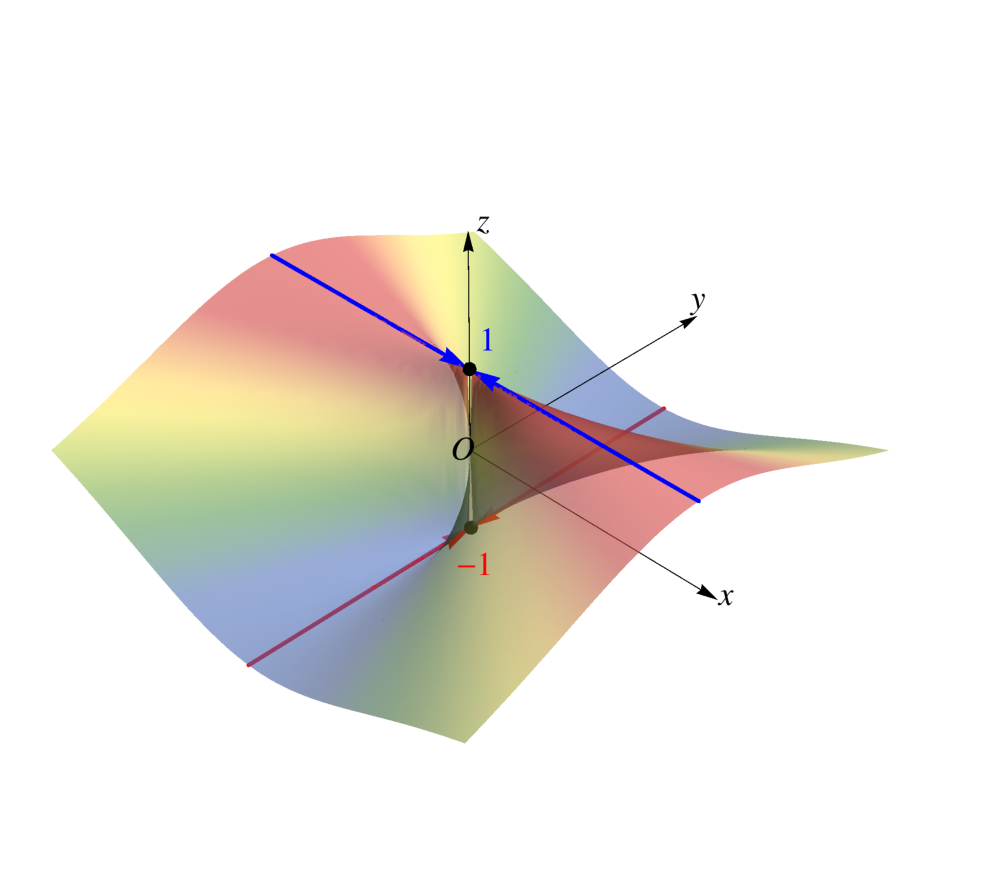
\includegraphics{./images/ch10/3DSurfaceLim-2-2.pdf}}
\end{center}

[提示]:若{\bf 累次极限}
$$\lim\limits_{y\to y_0}\lim\limits_{x\to x_0}f(x,y),
\quad \lim\limits_{x\to x_0}\lim\limits_{y\to y_0}f(x,y)$$
不相同,或者某个累次极限不存在,则二重极限不存在。原因如下:
\begin{enumerate}[(1)]
  \setlength{\itemindent}{1cm}
  \item 二重极限相当于从$(x,y)$出发,沿着$(x,y)\to(x_0,y)\to(x_0,y_0)$
  或$(x,y)\to(x,y_0)\to(x_0,y_0)$的“折线”路径趋于$(x_0,y_0)$
  \item 二重极限与累次极限的关系:
  \begin{itemize}
    \item {\kaishu 若三者都存在,则相等}
    \item {\kaishu 二重极限存在,累次极限必存在} 
    \item {\kaishu 两个累次极限均存在且相等,二重极限未必存在}
  \end{itemize}
\end{enumerate}

% \begin{center}
% 	\resizebox{!}{4cm}{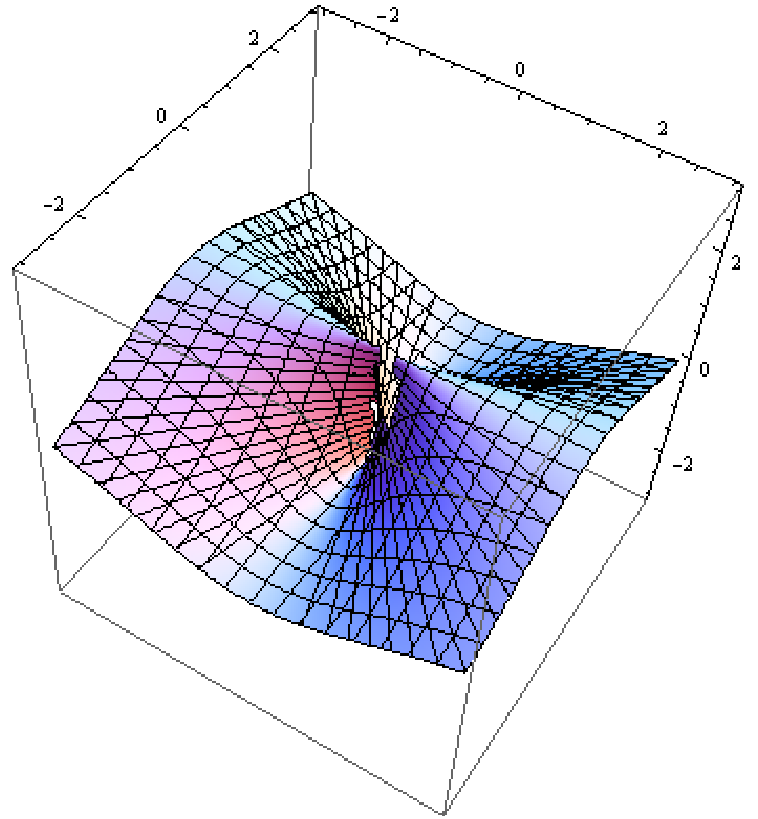
\includegraphics{./images/ch10/noLimEx.pdf}}
% 	\quad
% 	\resizebox{!}{4cm}{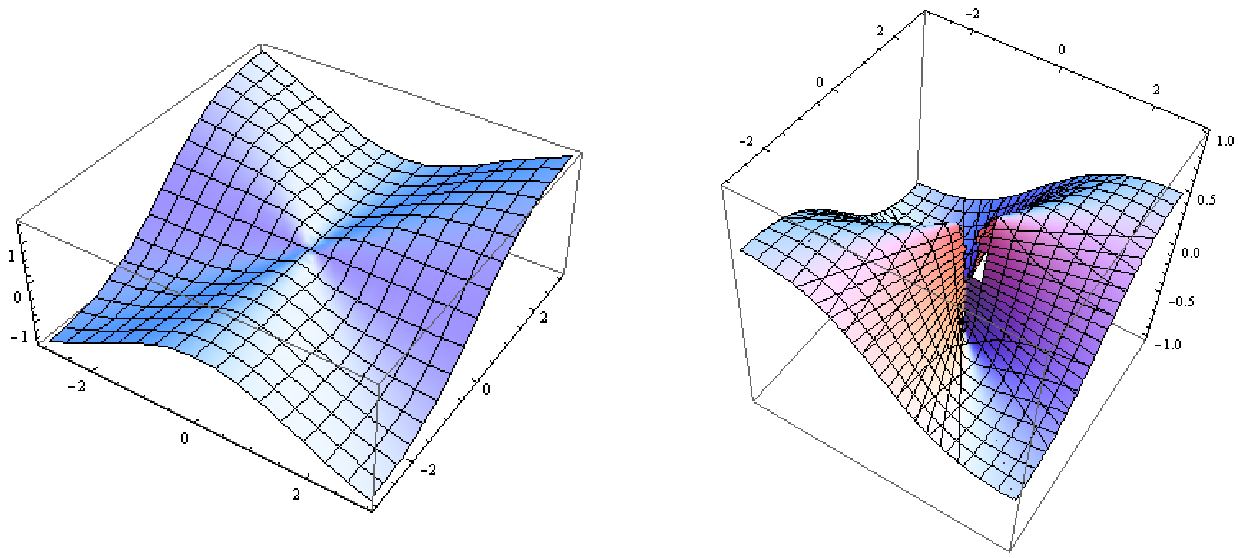
\includegraphics{./images/ch10/limEx.pdf}}
% 	
% 	教材-图10.1.13\hspace{2cm} 教材-图10.1.14\hspace{2cm} 教材-图10.1.15
% \end{center}

{\bf 例:}证明极限$\lim\limits_{(x,y)\to(0,0)}\df{xy}{x^2+y^2}$不存在

\begin{center}
	\resizebox{!}{4cm}{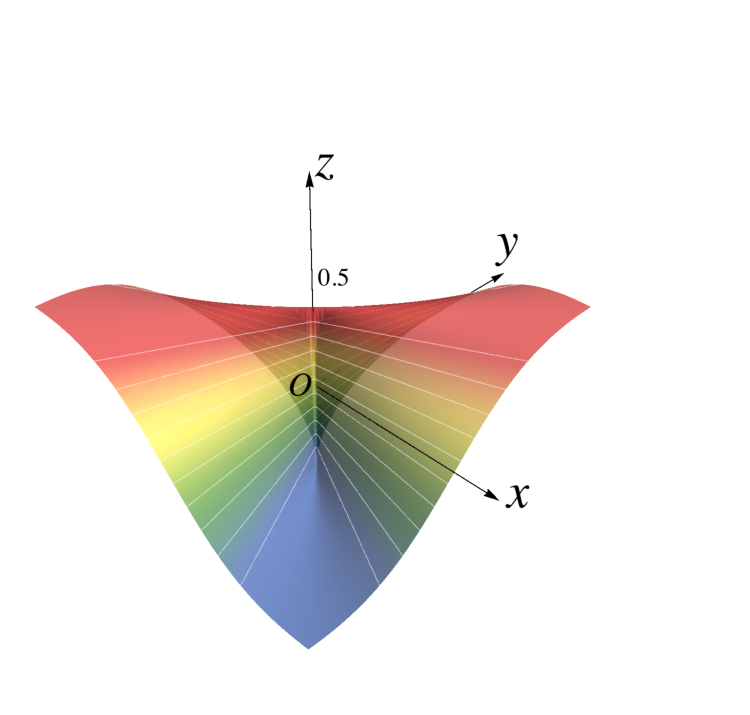
\includegraphics{./images/ch10/3DSurfaceLim-1-1.pdf}}
	\quad
	\resizebox{!}{4cm}{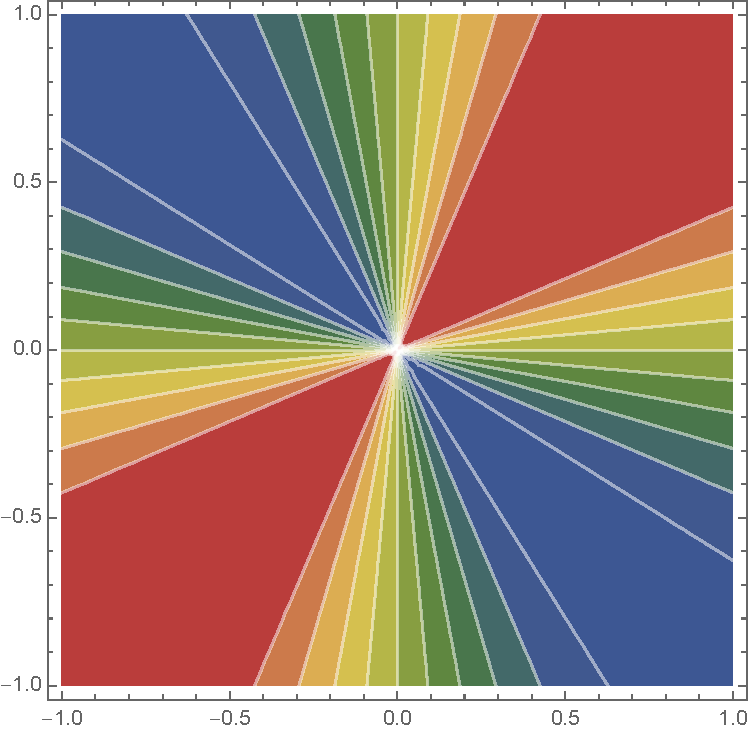
\includegraphics{./images/ch10/3DSurfaceLim-1-3.pdf}}
	\quad
	\resizebox{!}{4cm}{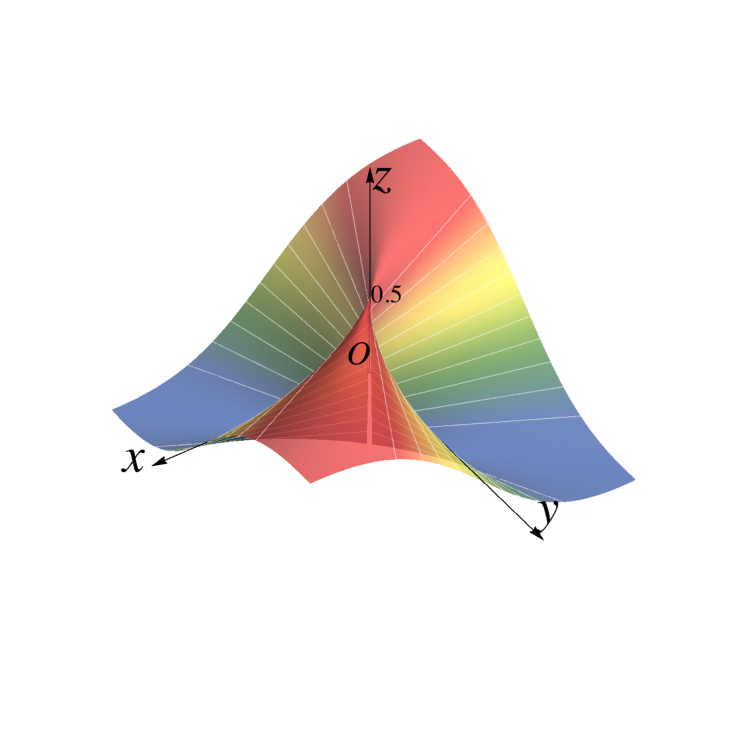
\includegraphics{./images/ch10/3DSurfaceLim-1-2.pdf}}
\end{center}

[提示]:若极限
$$\lim\limits_{{x\to x_0}\atop{y=y_0+k(x-x_0)}}f(x,y)$$
与$k$有关,则二重极限不存在。

沿着$y-y_0=k(x-x_0)$令$x\to0$,相当于从某个$(x,y)$出发,沿着直线趋于$(x_0,y_0)$。

以上两个例子中分别使用了两种不同的路径讨论二元函数极限的存在性问题,
无论是其中哪一种,其中所涉及的都只是各种可能的趋近路径中的一小部分,
并不能代表所有的情况,因此,这两种套路只能用于证明二重极限不存在。

证明二重极限不存在,只要找到不同的趋近路线,然后说明其上对应的极限不同即可,
这种思路类似于利用Hiene定理证明某些一元函数的极限不存在。显然,要证明某个
二重极限,我们不可能逐条验证所有的趋近路线,因此,很多时候只能回到“出发点”,
也就是利用利用二重极限的定义本身来进行证明。

{\bf 例:}$\lim\limits_{(x,y)\to(0,0)}\df{x^2y}{x^2+y^2}$

\begin{center}
	\resizebox{!}{4cm}{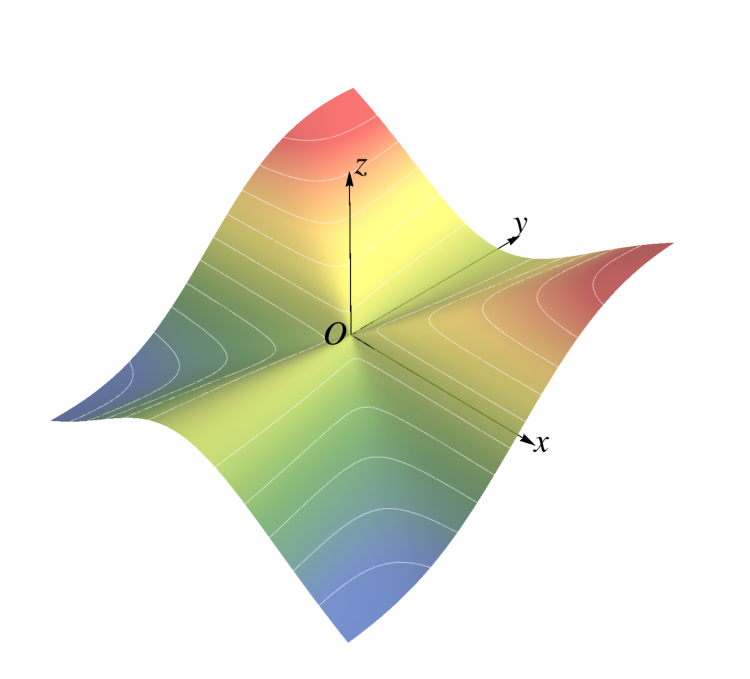
\includegraphics{./images/ch10/3DSurfaceLim-3-1.pdf}}
	\quad
	\resizebox{!}{4cm}{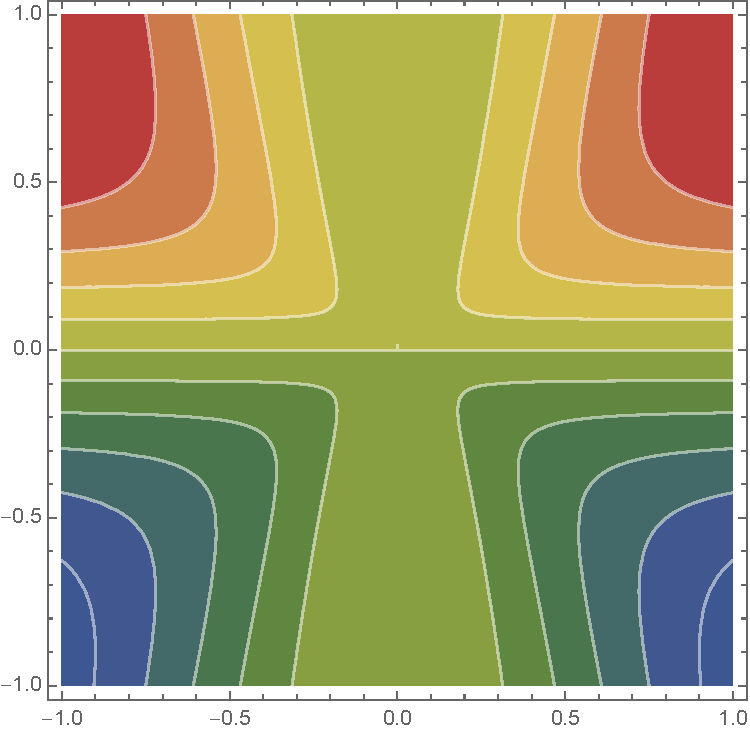
\includegraphics{./images/ch10/3DSurfaceLim-3-2.pdf}}
\end{center}

[提示]:令$x=x_0+\rho\cos\theta,y=y_0+\rho\sin\theta$,则
$$(x,y)\to(x_0,y_0)\quad\Leftrightarrow\quad\rho\to0$$
此时若极限
$$\lim\limits_{\rho\to{0^+}}f(\rho\cos\theta,\rho\sin\theta)$$
{\it 一致收敛},则对应二重极限存在。这里所谓前述极限一致收敛,是指:存在常数$A$,
对任意$\e>0$,存在与$\theta$无关的$\delta>0$\ps{$\delta$的取值与},
对任意$\rho\in(0,\delta)$,恒有$|f(\rho\cos\theta,\rho\sin\theta)-A|<\e$。

讨论前述上述极限时,不能简单地将$\theta$视为常数(否则就相当于令$y=y_0+(x-x_0)\tan\theta$
的直线方向趋近目标),而是应该认为即使$\theta$是(任意一个)与$\rho$相关的函数,亦可保证
收敛到相同的极限。

{\bf 例:}\ps{辅导书(下)-P12-例6-6}讨论极限
$$\lim\limits_{(x,y)\to(0,0)}\df{xy^2}{x^2+y^4}$$
的存在性。

\begin{center}
	\resizebox{!}{4cm}{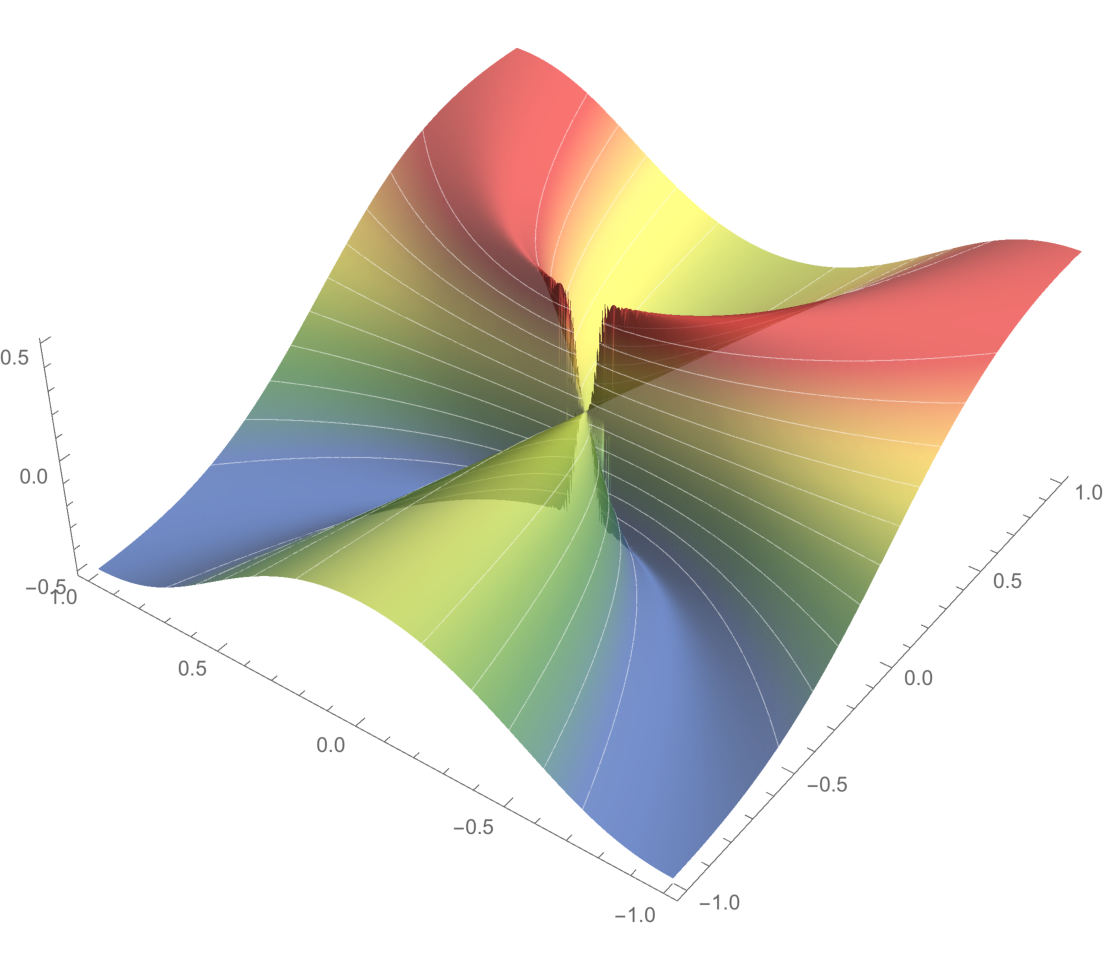
\includegraphics{./images/ch10/3DSurfaceLim-4-1.pdf}}
	\quad
	\resizebox{!}{4cm}{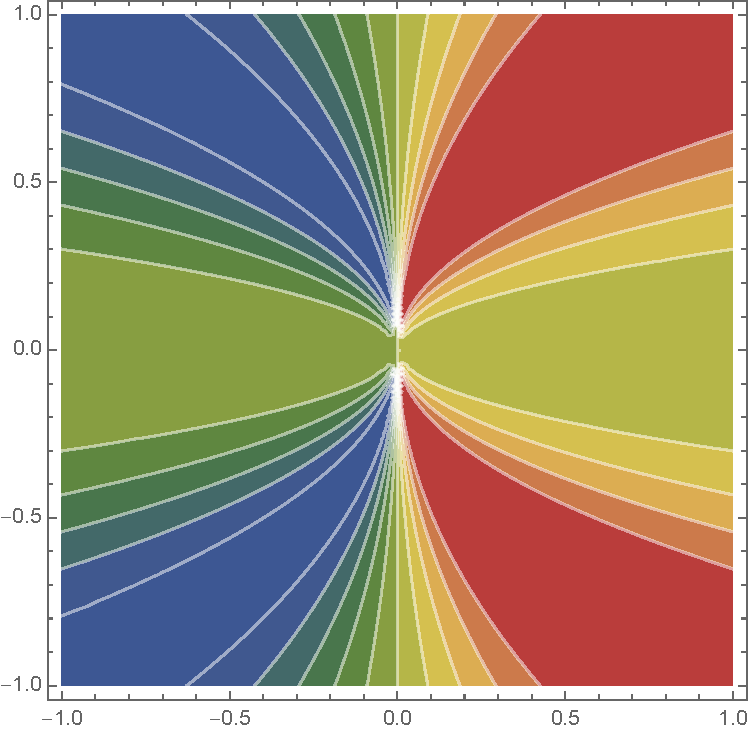
\includegraphics{./images/ch10/3DSurfaceLim-4-2.pdf}}
\end{center}

[证]:令$x=\rho\cos\theta,y=\rho\sin\theta$,则
$$\lim\limits_{(x,y)\to(0,0)}\df{xy^2}{x^2+y^4}
=\lim\limits_{\rho\to0^+}\df{\rho\cos\theta\sin^2\theta}
{\cos^2\theta+\rho^2\sin^4\theta}$$
我们可以证明,右端的极限不是一致收敛的。

显然,$\cos\theta=0$时,右端极限为$0$。

设$\cos\theta\ne 0$,则
$$\lim\limits_{\rho\to0^+}\df{\rho\cos\theta\sin^2\theta}
{\cos^2\theta+\rho^2\sin^4\theta}
=\lim\limits_{\rho\to0^+}\df{\rho\sin^2\theta}{\cos\theta},$$
对任意$k\in\mathbb{R},$若$\rho$和$\theta$满足
$\df{\rho\sin^2\theta}{\cos\theta}=k$,也即
$\rho^2\sin^2\theta=k\rho\cos\theta$,也即$ky^2=x$时,
则有
$$\lim\limits_{\rho\to0^+}\df{\rho\sin^2\theta}{\cos\theta}=k,$$
极限值与$k$有关,由此可见,原二重极限不存在。\fin

{\bf 例:}证明:$\lim\limits_{(x,y)\to(0,0)}\df{x^2y^2}{x^2+y^2}=0$
	
[证]:令$\rho=\sqrt{x^2+y^2}$,$\tan\theta=\df yx$,则	
$$\lim\limits_{(x,y)\to(0,0)}\df{x^2y^2}{x^2+y^2}
=\lim\limits_{\rho\to{0^+}}\rho^2\cos^2\theta\sin^2\theta$$
对任意$\e>0$,令$\delta=\sqrt{\e}$,则对任意$\rho\in(0,\delta)$,总有
$$|\rho^2\cos^2\theta\sin^2\theta|<\e,$$
从而可知原二重极限存在,且为$0$。\fin

% \begin{shaded}
% 	{\bf 二重极限与累次极限}
% 	
% 	{\bf 二重极限:}
% 	
% 	$$\lim\limits_{(x,y)\to(x_0,y_0)}f(x,y)$$
% 	
% 	{\bf 累次极限:}
% 	
% 	
% 	
% 	\begin{enumerate}[(1)]
%   	  \setlength{\itemindent}{1cm}
% 	  \item 若三者都存在,则值相等
% 	  \item 二重极限存在,累次极限必存在 
% 	  \item 两个累次极限均存在且相等,二重极限未必存在
% 	\end{enumerate}
% 	
% 	{\bf 思考:}如何从几何上解释三者之间的关系?
% 	
% 	\bigskip
% 	
% 	{\bf 关于用极坐标变换判定二重极限的存在性}
% 	
% 	讨论$\lim\limits_{(x,y)\to(x_0,y_0)}f(x,y)$
% 	的存在性时,可以令
% 	$$\rho=\sqrt{(x-x_0)^2+(y-y_0)^2},\quad \tan\theta=\df {y-y_0}{x-x_0},$$
% 	则
% 	$$(x,y)\to(x_0,y_0)\;\Leftrightarrow\;\rho\to0^+,$$
% 	从而
% 	$$\lim\limits_{(x,y)\to(x_0,y_0)}f(x,y)=\lim\limits_{\rho\to{0^+}}
% 	f(\rho\cos\theta,\rho\sin\theta).$$
% 	若右侧极限在$\rho\to{0^+}$的过程中与$\theta$的取值无关,则可以判定原极限存在。但
% 	要注意的是,这里不仅要求对任何固定的$\theta$(相当于沿着某条直线$y-y_0=k(x-x_0)$
% 	趋近$(x_0,y_0)$)	在$\rho\to{0^+}$时的极限与$\theta$无关,
% 	{\it 而且要求在$\rho\to{0^+}$过程中$\theta$可以随$\rho$的改变而取不同的值的情况
% 	下(例如沿着某条曲线$\rho=\rho(\theta)$趋近$(x_0,y_0)$)仍然无关,
% 	才能说明原极限存在。}
% 	
% 	{\bf 例:}证明:$\lim\limits_{(x,y)\to(0,0)}\df{xy}{x+y}$不存在
% 	
% 	{\bf 证:}令$\rho=\sqrt{x^2+y^2}$,$\tan\theta=\df yx$,则
% 	$$\lim\limits_{(x,y)\to(0,0)}\df{xy}{x+y}
% 	=\lim\limits_{\rho\to{0^+}}\df{\rho\cos\theta\sin\theta}
% 	{\cos\theta+\sin\theta}
% 	$$
% 	\begin{center}
% 		\resizebox{!}{6cm}{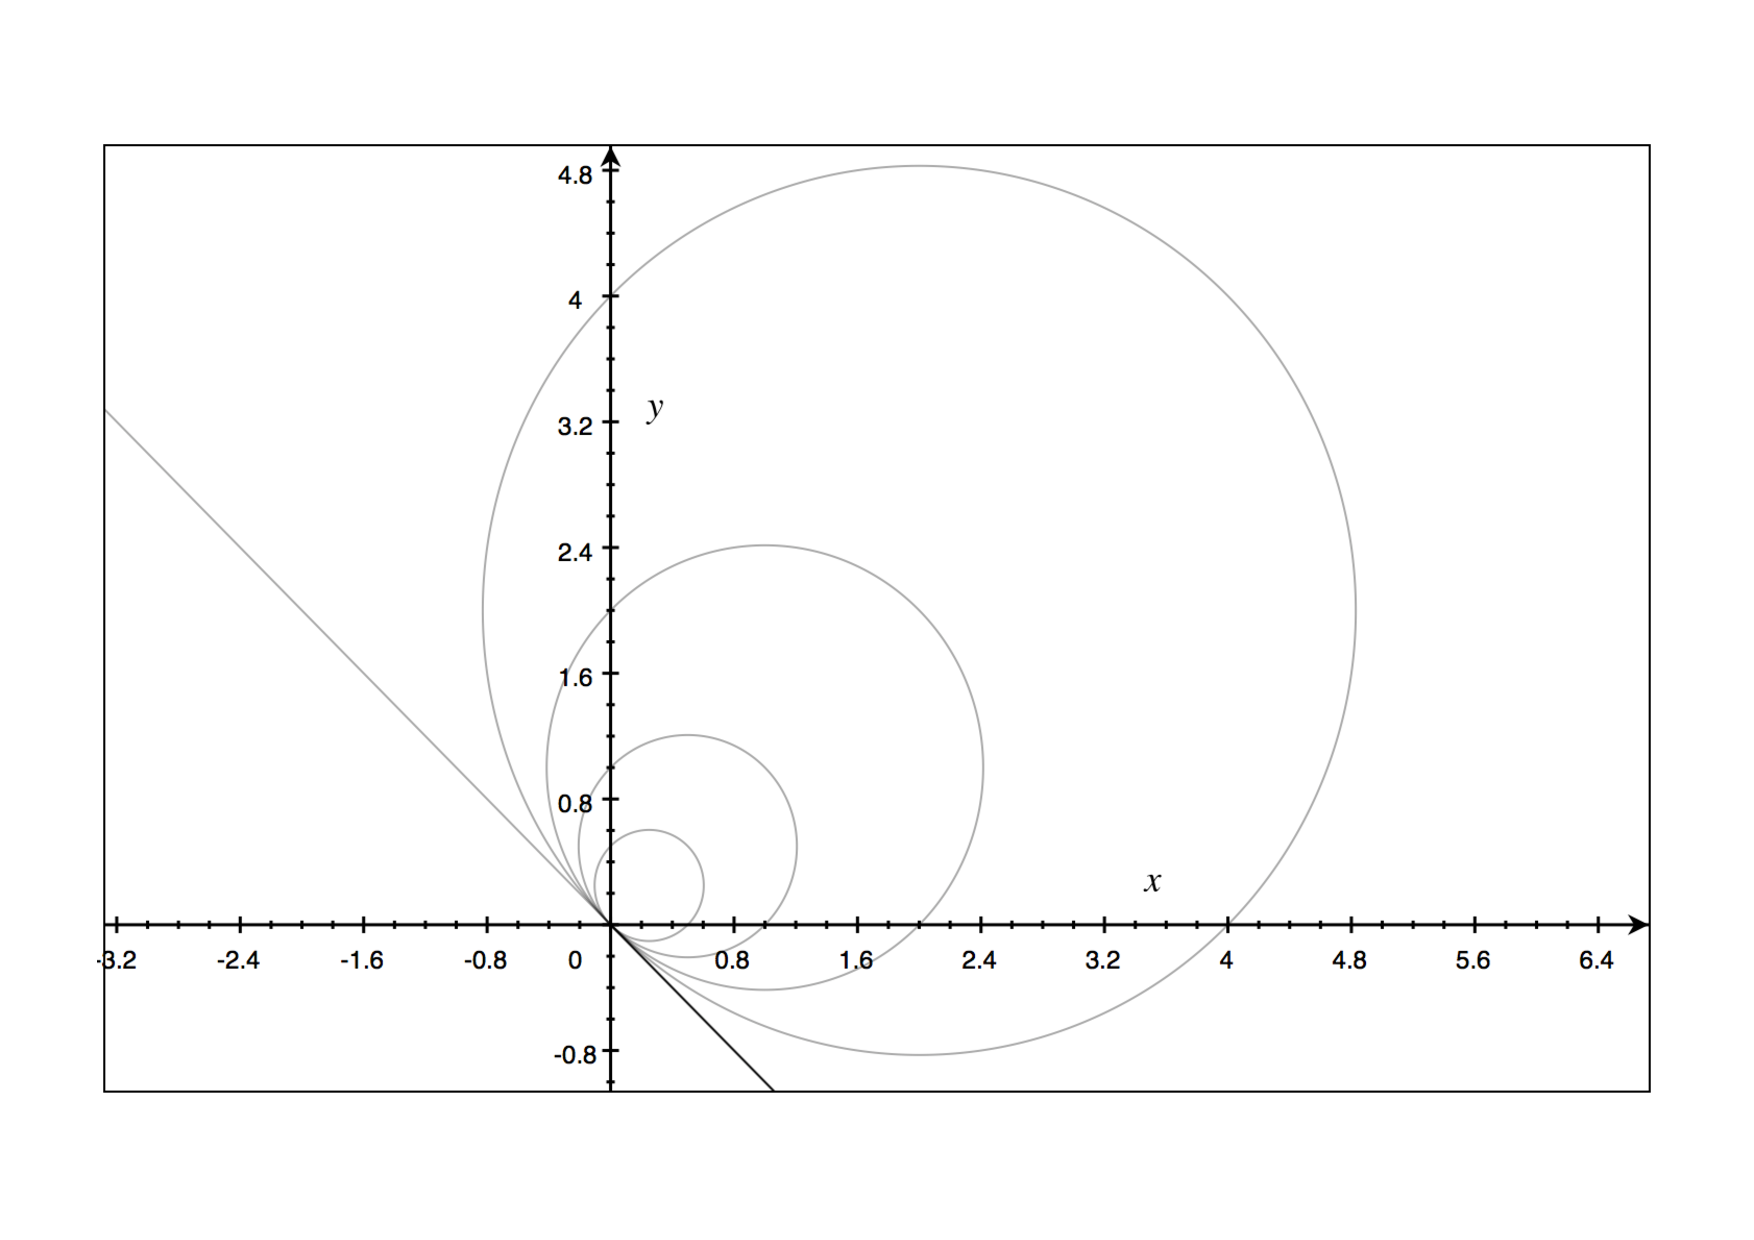
\includegraphics{./images/ch10/xy-xy.pdf}}
% 	\end{center}
% 	如图,考虑$(x,y)$沿$\rho=k(\cos\theta+\sin\theta)$趋于$(0,0)$,则
% 	当$\theta\to-\df{\pi}4$时,$\rho\to 0^+$,若原极限存在,则
% 	$$\lim\limits_{(x,y)\to(0,0)}\df{xy}{x+y}
% 	=\lim\limits_{\rho\to{0^+}}\df{\rho\cos\theta\sin\theta}
% 	{\cos\theta+\sin\theta}=\lim\limits_{\theta\to-\frac{\pi}4}
% 	k\cos\theta\sin\theta=-\df k2$$
% 	也即对应于不同的$k$值,极限计算的结果是不同的,故原极限不存在。
% 	
% 	{\bf 例:}证明:$\lim\limits_{(x,y)\to(0,0)}\df{x^2y^2}{x^2+y^2}=0$
% 	
% 	{\bf 证:}令$\rho=\sqrt{x^2+y^2}$,$\tan\theta=\df yx$,则	
% 	$$\lim\limits_{(x,y)\to(0,0)}\df{x^2y^2}{x^2+y^2}
% 	=\lim\limits_{\rho\to{0^+}}\rho^2\cos^2\theta\sin^2\theta$$	
% 	因为$\cos^2\theta\sin^2\theta\leq1$,故易知右侧极限与$\theta$无关且等于$0$,
% 	从而原极限等于$0$。
% 
% \end{shaded}

总结一下以上的分析思路,可以得到如下的具有一定通用性的判断方法:
\begin{thx}
	{\bf 判断二重极限$\lim\limits_{(x,y)\to(x_0,y_0)}f(x,y)$的存在性:}
	
	令$x=x_0+\rho\cos\theta,y=y_0+\sin\theta$,则
	$$\lim\limits_{(x,y)\to(x_0,y_0)}f(x,y)
	=\lim\limits_{\rho\to0}f(x_0+\rho\cos\theta,y_0+\rho\sin\theta).$$
	\begin{enumerate}[(1)]
	  \item 将$\theta$视为常数,若右端极限与$\theta$有关(即对$\theta$不同的取值,
	  极限不同),则原二重极限不存在;
	  \item 若存在$A$,使对任意$\e>0$,总存在与$\theta$无关的$\delta>0$,当
	  $0<|\rho|<\delta$时,有$|f(x_0+\rho\cos\theta,y_0+\rho\sin\theta)-A|<\e$,
	  则原二重极限存在,且为$A$。
	\end{enumerate}
\end{thx}

\subsection{多元函数的连续性}

\begin{thx}
	{\bf $n$元函数$f(\bm{x})$在$\bm{x}_0$处连续:}
	$f(\bm{x}_0)=\lim\limits_{\bm{x}\to\bm{x}_0}f(\bm{x})$
\end{thx}

\begin{thx}
	{\bf 定理:}多元初等函数在其定义区域内连续。
\end{thx}

{\bf 例:}求函数$f(x,y)=\df{\arcsin(3-x^2-y^2)}{\sqrt{x-y^2}}$连续的区域。

直接推广有界闭区间上连续的一元函数的性质,可得:
\begin{thx}
	{\bf 有界闭区域上连续函数的性质:}设$D\in\mathbb{R}^2$为有界闭区域,
	$f(x,y)$在$D$上连续,则
	\begin{enumerate}
% 	  \setlength{\itemindent}{1cm}
	  \item $f(x,y)$必在$D$上有界;
	  \item $f(x,y)$必在$D$上取到最大$M$和最小值$m$;
	  \item 对于介于$M$和$m$之间的任意实数$c$,必存在$(\xi,\eta)\in{D}$,使得
	  $f(\xi,\eta)=c$。
	\end{enumerate}
\end{thx}

\begin{ext}
	{\bf 课后作业}
	\begin{enumerate}
	  \item 讨论以下二重极限的存在性
	  \begin{enumerate}[(1)]
	    \item $\lim\limits_{(x,y)\to(0,0)}\df{x+y}{\sqrt{x^2+y^2}}$
% 	    \item $\lim\limits_{(x,y)\to(0,0)}\df{y^2+\sin x}{y^2+x}$
	    \item $\lim\limits_{(x,y)\to(0,0)}\df{xy}{|x|+|y|}$
	  \end{enumerate}
	  \item 计算以下二重极限
	  \begin{enumerate}[(1)]
	    \item $\lim\limits_{(x,y)\to(0,1)}\df{\ln(1+xy)}{y\sin x}$
	    \item $\lim\limits_{(x,y)\to(0,0)}\df{1-\cos(xy)}{(x^2+y^2)e^{x^2}}$
	    \item $\lim\limits_{(x,y)\to(0,0)}\df{e^{xy}-1}{\sqrt{2-e^{xy}}-1}$
	  \end{enumerate}
	\end{enumerate}
\end{ext}

\section{偏导数与全微分}

\subsection{偏导数}

\begin{thx}
{\bf 二元函数$z=f(x,y)$在$(x_0,y_0)$处关于$x$的偏导数:}
$$
	f'_x(x_0,y_0)
	 =  \lim\limits_{\Delta x\to 0}\df{f(x_0+\Delta x,y_0)-f(x_0,y_0)}
	 {\Delta x} 
	=\left.\df{\d}{\d x}f(x,y_0)\right|_{x=x_0} 
	 =  {\left.\df{\p z}{\p x}\right|_{x=x_0,y=y_0}}
$$
\end{thx}
由定义不难看出,偏导数等价于将其他变量视为常数所求得的导数。

{\bf 例:}已知$f(x,y)=x^2+2xy$,求$f'_x(-1,1)$和$f'_y(-1,1)$。

\begin{thx}
	{\bf 偏导数的几何意义:}$f'_x(x_0,y_0)$表示空间曲线
	$$\left\{\begin{array}{l}
	z=f(x,y)\\ y=y_0
	\end{array}\right.$$
	在点$(x_0,y_0,f(x_0,y_0))$处的切线相对于$x$轴的斜率。
	\begin{center}
		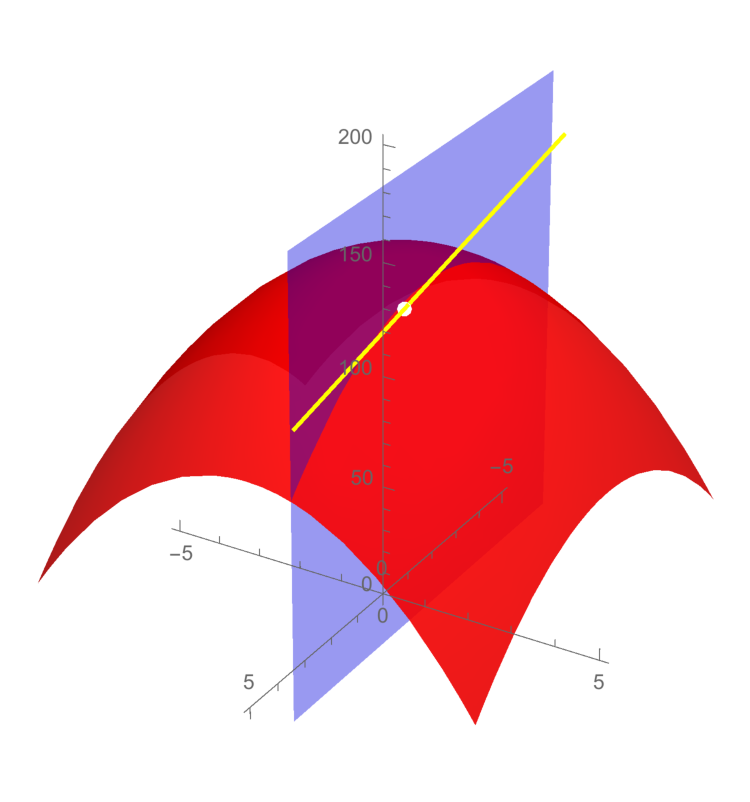
\includegraphics[width=0.35\textwidth]{./images/ch9/px.pdf}\quad
		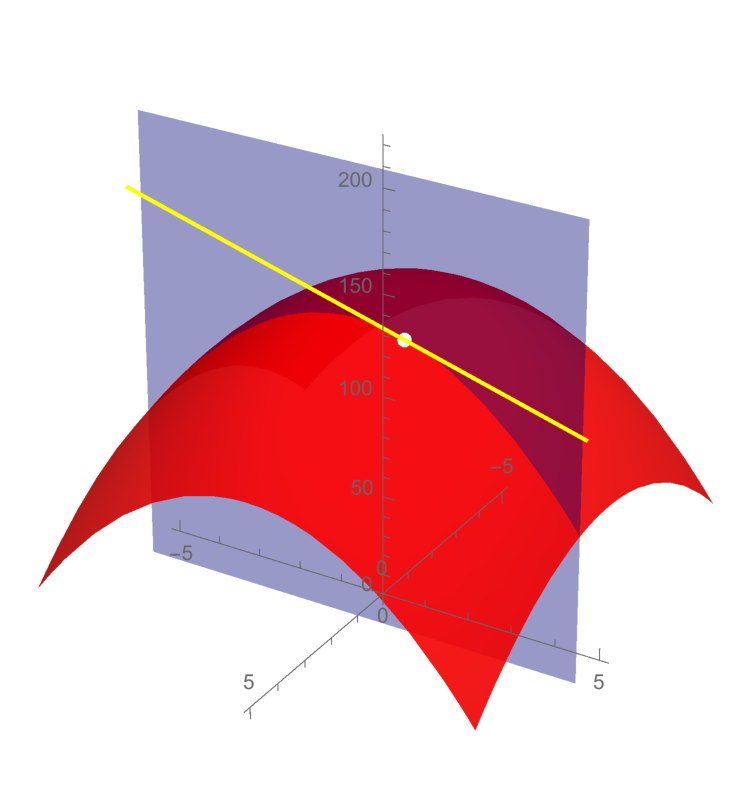
\includegraphics[width=0.35\textwidth]{./images/ch9/py.pdf}
	\end{center}
\end{thx}

{\bf 例:}$f(x,y)=\left\{\begin{array}{cc}
	\df{xy}{x^2+y^2}, & (x,y)\ne (0,0)\\
	0, & else
\end{array}\right.$
求$f'_x(0,0)$和$f'_y(0,0)$

这个例子告诉我们:{\kaishu 多元函数在一点偏导数存在,未必在该点连续!}
这一点和一元函数(可导必连续)是不同的。

\subsection{偏导数的计算}

运算规则:对指定变量求导时,将其他变量视为常数!

{\bf 例:}求以下函数的各个偏导数
\begin{enumerate}[(1)]
  \setlength{\itemindent}{1cm}
  \item $z=x^y$
  \item 已知$r=\sqrt{x^2+y^2+z^2}$,证明
	$$\left(\df{\p r}{\p x}\right)^2+\left(\df{\p r}{\p y}\right)^2+\left(\df{\p
	r}{\p z}\right)^2=1$$
\end{enumerate}

\subsection{高阶偏导数}

{\bf 二阶偏导数:}偏导数的偏导数 
$${f''_{xx}(x,y)=\df{\p}{\p x}\left(\df{\p z}{\p x}\right)
=\df{\p^2 z}{\p x^2}}$$ 
$${f''_{xy}(x,y)=\df{\p}{\p y}\left(\df{\p z}{\p x}\right)
=\df{\p^2 z}{\p x\p y}}$$ 
$${f''_{yy}(x,y)=\df{\p}{\p y}\left(\df{\p z}{\p y}\right)
=\df{\p^2 z}{\p y^2}}$$ 
$${f''_{yx}(x,y)=\df{\p}{\p x}\left(\df{\p z}{\p y}\right)
=\df{\p^2 z}{\p y\p x}}$$

{\bf 例:}验证函数$u=\sin(x-at)$满足{\bf 波动方程}
$\df{\p^2u}{\p t^2}=a^2\df{\p^2u}{\p x^2}$

\begin{thx}
	{\bf 定理:}若函数$z=f(x,y)$的两个混合偏导函数$f''_{xy}(x,y)$
	和$f''_{yx}(x,y)$均在$(x_0,y_0)$处连续,则
	$$f''_{xy}(x_0,y_0)=f''_{yx}(x_0,y_0)$$
\end{thx}

显然,该定理的结论可推广到高阶偏导数的情形。

该定理意味着,在一定条件下,函数的高阶偏导数可以选择任意的次序。特别地,
对初等函数而言,求高阶偏导数的结果总是与求导的次序无关的。

\subsection{全微分}

\begin{shaded}
	{\bf 一元函数$y=f(x)$在$x_0$处的微分}
	
	\begin{enumerate}[(1)]
  	  \setlength{\itemindent}{1cm}
  	  \item {\bf 局部线性化(以直代曲):}在$x_0$附近,切线上的函数值近似$f(x)$的函数值,
  	  也即
  	  $$f(x_0+\Delta x)\approx f(x_0)+f'(x_0)\Delta x;$$
	  \item {\bf 可微:}存在常数$A$,使得
	  $$\Delta y=A\Delta x+\circ(\Delta x)$$
	  \item {\bf 微分:}$\d y|_{x=x_0}=A\Delta x=f'(x_0)\Delta x=f'(x_0)\d x$
	\end{enumerate}
\end{shaded}

\subsubsection{二元函数的局部线性化}

{\bf 问题:}对于二元(或者多元)函数, 
\begin{itemize}
  \item 在什么情况下,存在类似的近似?
  \item 如何表达这样的近似? 
  \item 这种近似蕴含了哪些性质?
\end{itemize}

不难看出,切平面是平面上切线概念在三维空间中的推广,因此,所谓
对二元函数的局部线性化(或以直代曲),也即在$(x_0,y_0)$附近
用切平面上的函数值近似替代$f(x,y)$的函数值。

{\bf 例:}求椭圆抛物面$S:z=2x^2+3y^2$在点$P(1,1,5)$处的切平面方程。

\begin{center}
	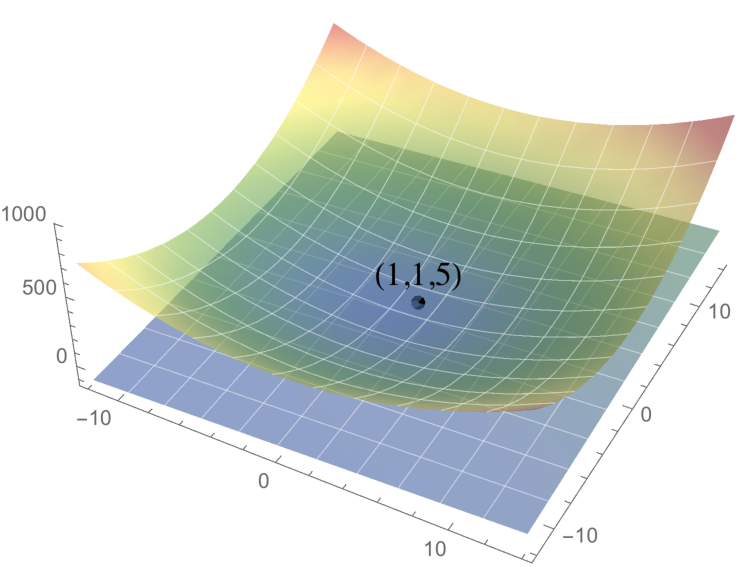
\includegraphics[width=0.3\textwidth]{./images/ch10/3DSurfaceDeri-1-1.pdf}
	\quad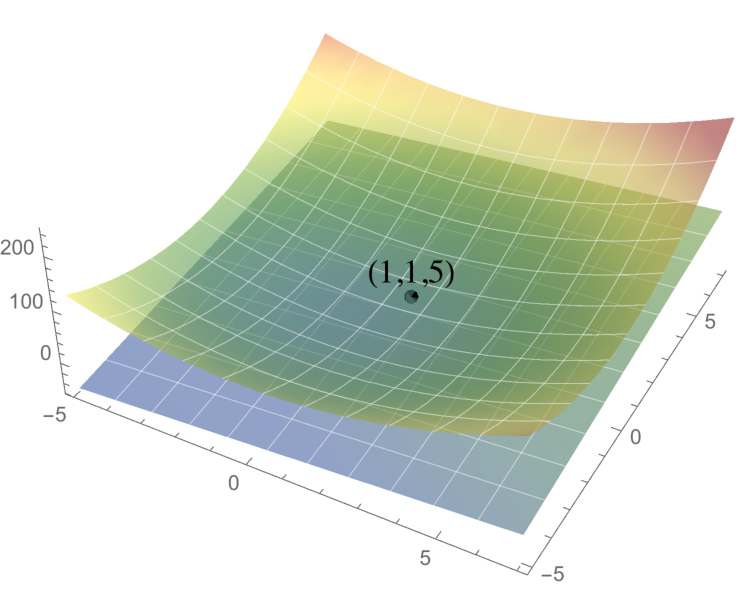
\includegraphics[width=0.3\textwidth]{./images/ch10/3DSurfaceDeri-1-2.pdf}
	
	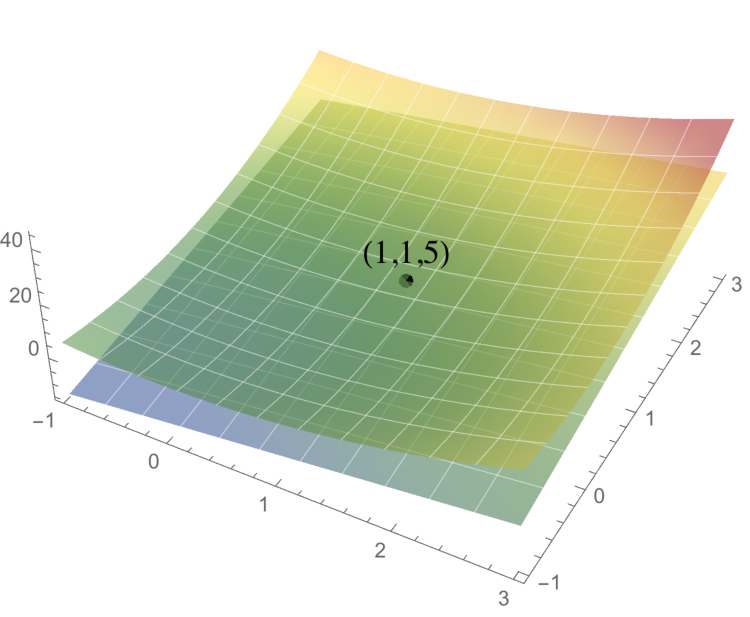
\includegraphics[width=0.3\textwidth]{./images/ch10/3DSurfaceDeri-1-3.pdf}
	\quad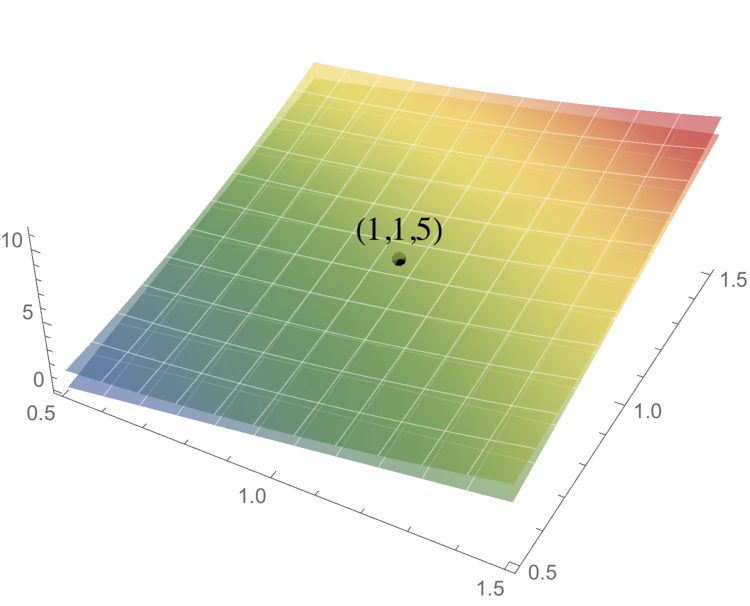
\includegraphics[width=0.3\textwidth]{./images/ch10/3DSurfaceDeri-1-4.pdf}
	
	{\it 越靠近切点,切平面与曲面的近似程度越高}
\end{center}

若函数$f(x,y)$在$(x_0,y_0)$处的偏导数都存在,则由其所对应的两条切线,
总是可以定义出曲面可能的切平面:
\begin{center}
	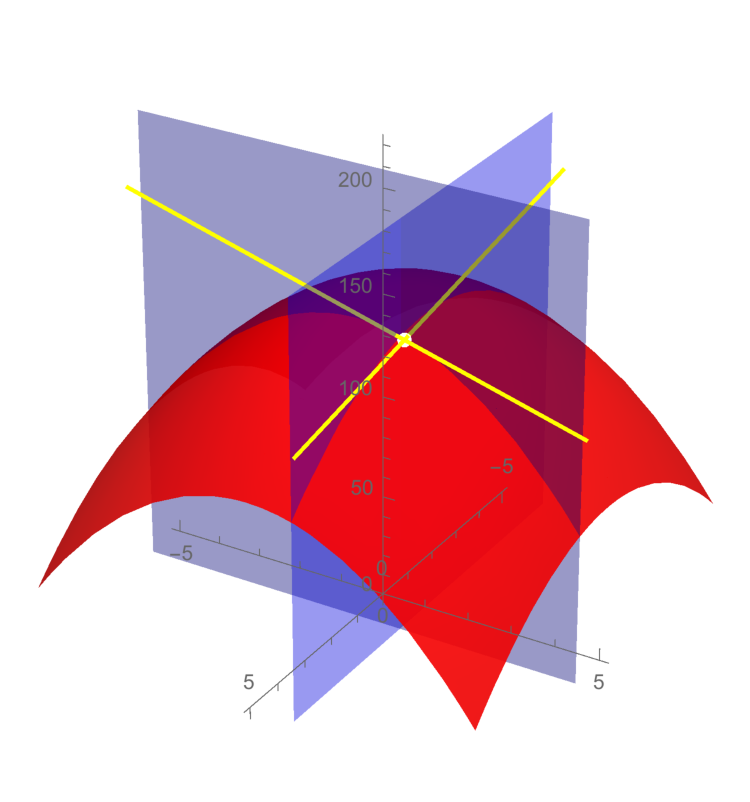
\includegraphics[width=0.35\textwidth]{./images/ch9/pxy.pdf}\quad
	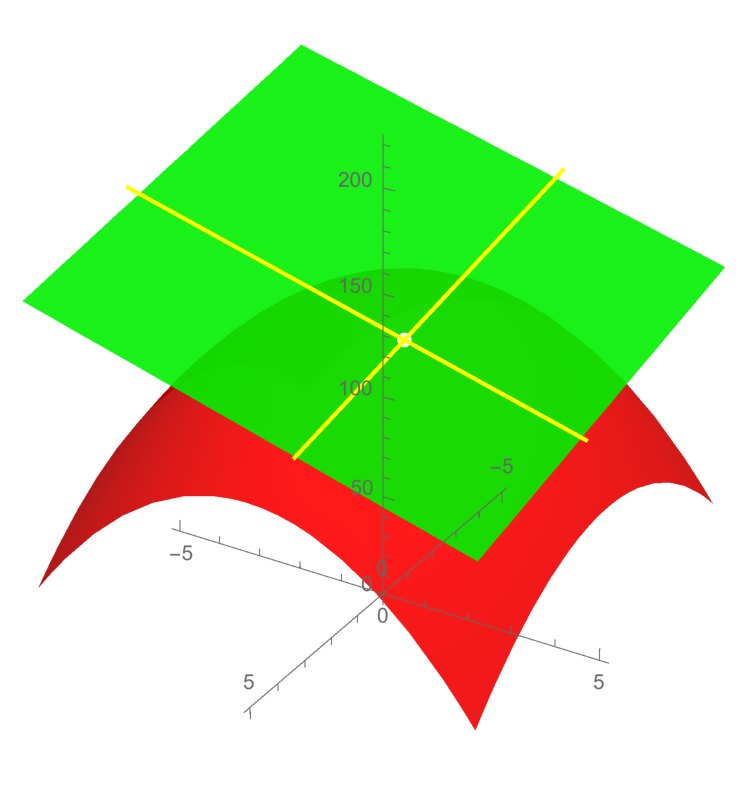
\includegraphics[width=0.35\textwidth]{./images/ch9/ppxy.pdf}
\end{center}

{\bf 例:}如果将切平面定义为沿$x$轴和$y$轴方向的两条切线所确定的平面,试
讨论函数
$$f(x,y)=\left\{\begin{array}{cc}
	\df{xy}{x^2+y^2},& (x,y)\ne (0,0)\\
	0, & else
\end{array}\right.$$
在原点处是否存在切平面?

[提示]:如图
\begin{center}
	\resizebox{!}{4.5cm}{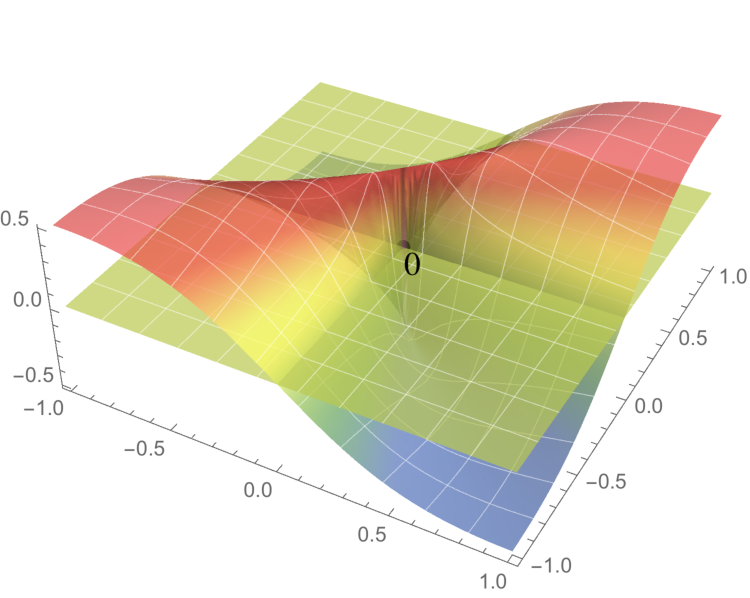
\includegraphics{./images/ch10/3DSurfaceDeri-2-1.pdf}}
	\quad\resizebox{!}{4.5cm}{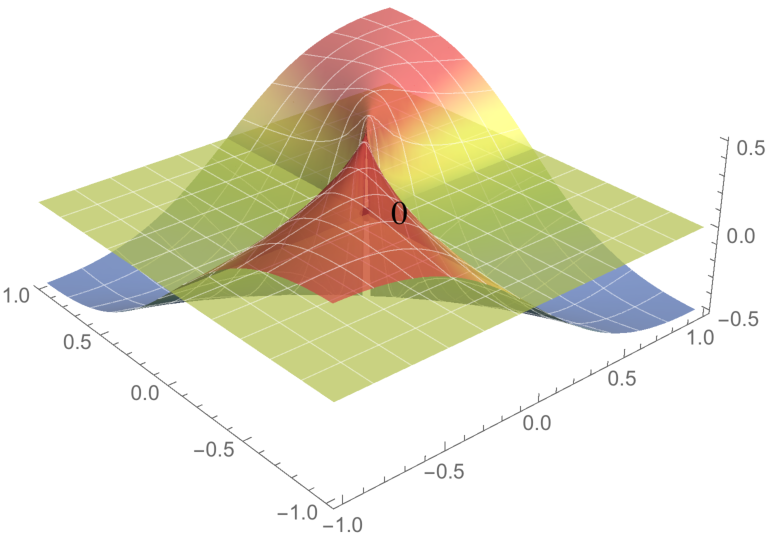
\includegraphics{./images/ch10/3DSurfaceDeri-2-2.pdf}}
	
	{\it 可能的“切平面”未必就是真正的切平面!}
\end{center}

\begin{thx}
	{\bf 切平面存在的必要条件:}
	$$f(x_0+\Delta x,y_0+\Delta y)\approx f(x_0,y_0)+f'_x(x_0,y_0)\Delta
	x+f'_y(x_0,y_0)\Delta y$$
\end{thx}

\subsubsection{全微分的概念}

以二元函数为例,
\begin{thx}
	  {\bf 函数$z=f(x,y)$在$(x_0,y_0)$处可微},是指:存在常数$A,B$,使得
	  $$\Delta z-A\Delta x-B\Delta y=\circ(\sqrt{(\Delta x)^2+(\Delta y)^2}).$$
	  相应地,{\bf 函数$z=f(x,y)$在$(x_0,y_0)$处的全微分}记为
	  $$\d z|_{(x_0,y_0)}=A\Delta x+B\Delta y.$$
\end{thx}

{\bf 例:}验证$z=2x^2+3y^2$在$(1,1,5)$处可微。

显然,可以类似地定义多元函数的全微分。

{\bf 例:}证明:三元函数$w(x,y,z)$的每个偏导数均为常数,当且仅当$w$为
$x,y,z$的线性函数。

\subsubsection{全微分的性质}

\begin{thx}
	\begin{enumerate}
	  \item 若多元函数在某点可微,则必在该点连续;
	  \item 若多元函数在某点可微,则必在该点处的偏导数均存在;
	  \item 对于可微的二元函数$z=f(x,y)$,
	  $$\d z=\df{\p z}{\p x}\Delta x+\df{\p z}{\p y}\Delta y,$$
	  或者更一般地写为
	  $${\d z=\df{\p z}{\p x}\d x+\df{\p z}{\p y}\d y}.$$ 
	\end{enumerate}
\end{thx}

{\bf 例:}验证:函数$f(x,y)=\left\{\begin{array}{cc}
	\df{xy}{x^2+y^2},& (x,y)\ne (0,0)\\
	0, & else
\end{array}\right.$
在原点处不连续,但偏导数均存在。

该例说明,即使偏导数都存在,也不能退出多元函数函数一定可微。
\ps{\b 与一元函数性质的重要差异!}

{\bf 例:}求$u=e^{x-y}+\sin z$在$(2,1,0)$处的全微分。

\begin{thx}
	{\bf 定理:}若二元函数$z=f(x,y)$在某点处的偏导函数
	$\df{\p z}{\p x}$和$\df{\p z}{\p y}$连续,则$f(x,y)$在该点可微。	
\end{thx}

显然,以上所有关于二元函数的结论都可以直接推广到$n$元函数的情形。

% \subsection*{小结}
% 
% \begin{enumerate}[(1)]
%   \setlength{\itemindent}{1cm}
%   \item {\bf 多元函数的极限与连续}
%   \begin{itemize}
%     \item 多重极限:沿任意路径逼近所得极限相同
%     \item 累次极限存在且相等,多重极限未必存在
%   \end{itemize}
%   \item {\bf 偏导数}
%   \begin{itemize}
%     \item 对指定变量求导时,将其他变量视为常数
%     \item 偏导存在,未必连续
%     \item 几何意义:沿某坐标轴方向的切线斜率
%   \end{itemize}
%   \item {\bf 高阶偏导}
%   \begin{itemize}
%     \item 初等函数的高阶偏导与求导次序无关
%   \end{itemize}
%   \item {\bf 全微分}
%   \begin{itemize}
%     \item 何时可以对曲面进行“以直代曲”?\hfill 可微$\Leftarrow$偏导函数连续
%     \item 对曲面“以直代曲”意味着什么?\hfill 曲面“光滑”$\Rightarrow$连续
%     \item 全微分的基本形式:${\d z=\df{\p z}{\p x}\d x+\df{\p z}{\p y}\d y}$
%     \hfill 全微分方程名称是怎么来的?
%   \end{itemize}
% \end{enumerate}
% 
% {\bf 思考:}为什么多元函数不能直接推广一元函数的导数定义呢?

{\bf 例:}证明函数
  $$f(x,y)=\left\{\begin{array}{cc}
  	\df{x^2y}{x^2+y^2},& (x,y)\ne (0,0)\\
  	0,& else
  \end{array}\right.$$
  在原点可微,但偏导数不连续。

{\bf 例:}证明:$z=\sqrt{|xy|}$在原点连续,偏导数存在,但不可微。

{\bf 例:}正六棱台的上下底和高分别为$1,2,2$,问
那个值的测量误差对其侧面积的值影响最大?

[提示]:设六棱台的上、下底长和高分别为$x,y,z$,在其侧面积
$$S=6\times\df12(x+y)\times\df12\sqrt{4z^2+3(y-x)^2}.$$
利用微分运算,可得
$$\d z|_{(1,2,2)}=S'_x(1,2,2)\Delta x+S'_y(1,2,2)\Delta y+
S'_z(1,2,2)\Delta z=\df3{\sqrt{19}}(5\Delta x+14\Delta y+12\Delta z)$$
由此可知$y$(下底长度)的测量误差对侧面积的值影响最大。

\begin{ext}
	{\bf 课后作业}
	\begin{enumerate}
% 	  \item 证明:函数$f(x,y)=\sqrt{|xy|}$在原点连续,偏导数存在,但不可微。
	  \item 证明:函数$f(x,y)=\left\{\begin{array}{ll}
	  	(x^2+y^2)\sin\df1{x^2+y^2}, & (x,y)\ne(0,0)\\
	  	0, & \mathrm{else}
	  \end{array}\right.$
	  的偏导数在原点处不连续,但$f(x,y)$在原点处可微。
	  \item 求$z=\arctan\df{x+y}{1-xy}$的所有二阶偏导数。
	  \item 已知$\df{\p z}{\p y}=\df{x^2+y^2}y$,$z(x,1)=e^x$,
	  求$z(x,y)\;(y\ne 0)$
	  \item 设$z=\dint_x^{xy}e^{(t-x)^2}\d t$,求$\df{\p z}{\p x}$和$\df{\p z}{\p y}$。
	  \item 求函数$z=xy^2$在$(1,2)$附近且$(\Delta x,\Delta y)=(0.1,-0.5)$时
	  对应的函数值的改变量(全增量)与全微分。
	  \item 利用微分计算$\sqrt{1.02+(1.97)^3}$的近似值。
	\end{enumerate}
\end{ext}

\section{多元复合函数与隐函数的偏导数}

\subsection{多元复合函数求导}

\begin{thx}
	{\bf 多元函数求导的链式法则:}
	设$z=f(u,v),u=u(x,y),v=v(x,y)$, 且相关偏导数均存在, 则有
	$${\df{\p z}{\p x}=\df{\p z}{\p u}\df{\p u}{\p x}
	+\df{\p z}{\p v}\df{\p v}{\p x}}$$
	$${\df{\p z}{\p y}=\df{\p z}{\p u}\df{\p u}{\p y}
	+\df{\p z}{\p v}\df{\p v}{\p y}}$$
\end{thx}

{\bf 注:}以上的求法法则可以形象地解释为:{\kaishu “嵌套”$\to$乘积,“并列”$\to$相加}

{\bf 例:}对下列函数分别求$\df{\p z}{\p x}$和$\df{\p z}{\p y}$
\begin{enumerate}[(1)]
  \setlength{\itemindent}{1cm}
  \item $z=e^u\cos v,u=2x-y,v=xy$
  \item $z=f(3x+2y,x^2+y^2)$
\end{enumerate}

% \begin{shaded}
% 	{\bf 一些典型的情况}
% 	\begin{enumerate}[(1)]
%   	  \setlength{\itemindent}{1cm}
% 	  \item $z=f(u,v),u=\varphi(x),v=\psi(x)$ 
% 	  \item $z=f(u,v,w),u=u(x,y),v=v(x,y),w=w(x,y)$ 
% 	  \item $z=f(u),u=\varphi(x,y)$ 
% 	  \item $z=f(x,u),u=\varphi(x,y)$
% 	\end{enumerate}
% \end{shaded}

{\bf 例:}设$z=f(x,x+y,x/y)$,其中$f$可微,求$\df{\p z}{\p x}$
和$\df{\p z}{\p y}$

{\bf 例:}设$z=f(x/y)$,其中$f$可微,证明:$x\df{\p z}{\p x}+y
\df{\p z}{\p y}=0$

{\bf 例:}设$z=xy+xf(x/y)$,其中$f$可微,证明:
$$x\df{\p z}{\p x}+y\df{\p z}{\p y}=xy+z$$

{\bf 例:}设$z=uv+\sin t,u=e^t,v=\cos t$,求$\df{\d z}{\d t}$

{\bf 例:}设$z=f(xy,x^2-y^2)$,其中$f$具有二阶连续偏导函数,
求$\df{\p^2 z}{\p x^2}$和$\df{\p^2 z}{\p x\p y}$

\subsection{一阶微分的形式不变性}

% {\bf 一元函数的一阶微分形式不变性:}对于一元函数$y=f(x)$,无论$x$是自变量
% 还是中间变量,其一阶微分形式都是
% $$\d y=f'(x)\d x$$

\begin{thx}
	{\bf 多元函数的微分形式不变性:}$z=f(\varphi(x,y),\psi(x,y))$的全微分
	$${\d z=\df{\p z}{\p x}dx+\df{\p z}{\p y}\d y
	=\df{\p z}{\p u}\d u+\df{\p z}{\p v}\d v}$$
	也即:{\kaishu 无论$u,v$是自变量还是中间变量,其所得到的微分表达形式都一样}
\end{thx}

利用一阶微分的形式不变性,可以通过求全微分的方法来求得一阶偏导数。特别地,关于
全微分的运算法则和一元函数中的微分运算法则并没有显著的差异:
\begin{thx}
	{\bf 微分的运算法则:}
	\begin{enumerate}[(1)]
	  \setlength{\itemindent}{1cm}
	  \item $\d(u\pm v)=\d u\pm \d v$
	  \item $\d(cu)=c\d u\;(C\in\mathbb{R})$
	  \item $\d(uv)=v\d u+u\d v$
	  \item $\d\left(\df uv\right)=\df{u\d v-v\d u}{v^2}$
	  \item $\d\left(\df 1v\right)=-\df{\d v}{v^2}$
	\end{enumerate}
\end{thx}

{\bf 例:}设$z=f(3x+2y,x^2+y^2)$,其中$f$可微,
求$\df{\p z}{\p x}$和$\df{\p z}{\p y}$

{\bf 例:}求$z=\arctan\df yx$的全微分和一阶偏导数。

{\bf 例:}设$z=f(x,x^2+y^2,x^2-y^2)$,其中$f$具有二阶连续偏导函数,
求$\df{\p^2 z}{\p x^2}$和$\df{\p^2 z}{\p x\p y}$

{\bf 例:}根据要求计算偏导数:
\begin{enumerate}[(1)]
  \setlength{\itemindent}{1cm}
  \item 设$z=u^2\ln v,u=\df xy,v=3x-2y$,求$\df {\p z}{\p x},\df{\p z}{\p
  y}$。
  \item 设$z=\arctan(xy),y=e^x$,求$\df{\d z}{\d x}$。
\end{enumerate}

{\bf 例:}设$f(u)$当$u>0$时二阶可导,且$z=f(\sqrt{x^2+y^2})$满足方程
$$\df{\p^2z}{\p x^2}+\df{\p^2z}{\p y^2}=0,$$
\begin{enumerate}[(1)]
  \setlength{\itemindent}{1cm}
  \item 证明:$uf''(u)+f'(u)=0$;
  \item 设$f(1)=0,f'(1)=1$,求$f(u)$。 
\end{enumerate}

[提示]:
$$z'_x=f'(u)\df xu,\quad z'_z=f'(u)\df yu,$$
$$z''_{xx}=\df1{u^2}\left(f''(u)x^2+f'(u)\df{y^2}u\right),$$
$$z''_{yy}=\df1{u^2}\left(f''(u)y^2+f'(u)\df{x^2}u\right).$$
解方程可得$f(u)=\ln|u|$.

{\bf 例:}设$u(x,y)$满足
$$\df{\p^2 u}{\p x^2}-\df{\p^2 u}{\p y^2}
+k\left(\df{\p u}{\p x}+\df{\p u}{\p y}\right)=0.$$
试选择合适的$a,b$,使得通过变换$u(x,y)=v(x,y)e^{ax+b}$后,所得
新的方程不再含有任何偏导数项。

\subsection{隐函数的偏导数}

一般的多元函数表达式,可以说是一种函数和自变量相分离(分别位于等号两边)
的表达形式,其优点是自变量和因变量有着明显的区分,便于进行函数值的计算。
但也正是因为这种显式的设定,一定程度上也限制了其表示能力。与之相对地,
隐函数方程中通常没有明确地确定哪些变量为自变量,哪些是函数,而更多地
可以将这种分别留待实际进行计算时来确定,从而也就很容易图片函数必须是
“一对一”或“一对多”的限定,具有更强的表达能力。

对于包含两个变量的隐函数,在求解与之相关的导数时,通常是这样做的:给定隐函数方程
$f(x,y)=0$,假设其满足各种求导条件,并且将$y$视为$x$的函数$y(x)$,于是
可以在隐函数方程两边同时关于$x$求导,进而得到
$$f'_x(x,y(x))+f'_y(x,y(x))y'(x)=0
\quad\Rightarrow
y'(x)=-\df{f'_x(x,y(x))}{f'_y(x,y(x))},$$
或者就写作
$$y'(x)=-\df{f'_x(x,y)}{f'_y(x,y)}.$$

接下来我们主要考虑形如
$$\left\{\begin{array}{l}
	  	x^2+y^2+z^2=4\\
	  	(x-1)^2+y^2=1
	  \end{array}\right.$$
的包含更多变量的隐函数方程或方程组,该如何求其相关(偏)导数的问题。
为此,首先需要确定隐函数中哪些变量时自变量,哪些是函数,换句话说,
首先要确定是求哪个变量关于哪个变量的(偏)导数。

\subsubsection{隐函数中的函数关系}

注意到这样的关系:
$$\mbox{\kaishu 自由度}=\mbox{\kaishu 空间的维度}-\mbox{\kaishu 约束的个数},$$
或者说
$$\mbox{\kaishu 自变量的个数}=\mbox{\kaishu 变量的个数}-\mbox{\kaishu 方程的个数},$$
我们总是可以根据所给的方程(组)自身的信息来确定自变量和函数的个数。例如
\begin{enumerate}
  \setlength{\itemindent}{1cm}
  \item 一个方程所确定的隐函数可能是 
  $$F(x,y)=0 \quad \Rightarrow \quad y=f(x) $$
  $$F(x,y,z)=0 \quad \Rightarrow \quad z=f(x,y) $$
  \item 方程组所确定的隐函数可能是 
  $$\left.\begin{array}{l}
  	F(x,y,z)=0\\ G(x,y,z)=0
  \end{array}\right\} \quad \Rightarrow \quad 
  \left\{\begin{array}{l}
  	y=f(x)\\ z=g(x)
  \end{array}\right. $$
\end{enumerate}

以下分别针对不同的隐函数方程形式讨论其中的求导问题:

\begin{thx}
	{\bf 隐函数存在定理I:}若函数$F(x,y)$满足: 
	\begin{enumerate}[(1)]
	  \setlength{\itemindent}{1cm}
	  \item $F(x_0,y_0)=0$ 
	  \item $F(x,y)$在$(x_0,y_0)$附近偏导数连续 
	  \item $F_y'(x_0,y_0)\ne 0$ 
	\end{enumerate}
	则:方程$F(x,y)=0$在$(x_0,y_0)$的某邻域内唯一确定一个函数$y=y(x)$,使得
	在$x_0$附近满足$F(x,f(x))=0$, 且
	$${\df{\d y}{\d x}=-\df{F'_x}{F'_y}}$$
\end{thx}

{\bf 例:}设$2^{xy}=x+y$,求$\df{\d y}{\d x}$

\begin{thx}
	{\bf 隐函数存在定理II:}
	若函数$F(x,y,z)$满足: 
	\begin{enumerate}[(1)]
	  \setlength{\itemindent}{1cm}
	  \item $F(x_0,y_0,z_0)=0$ 
	  \item $F(x,y,z)$在$(x_0,y_0,z_0)$附近偏导数连续 
	  \item $F_z'(x_0,y_0,z_0)\ne 0$ 
	\end{enumerate}
	则:方程$F(x,y,z)=0$在$(x_0,y_0,z_0)$的某邻域内唯一确定一个函数$z=z(x,y)$,使得
	在$(x_0,y_0)$附近满足$F(x,y,z(x,y))=0$, 且
	$$\df{\p z}{\p x}=-\df{F'_x}{F'_z},\df{\p z}{\p y}=-\df{F'_y}{F'_z}$$
\end{thx}

{\bf 例:}设$x^2+y^2+z^2=3xyz$,求$\df{\p z}{\p x},\df{\p z}{\p y}$

{\bf 例:}设$x^2y-e^z=z$,求$\df{\p z}{\p x},\df{\p z}{\p y}$
 和$\df{\p^2z}{\p x\p y}$
 
{\bf 例:}设$y=y(x),z=z(x)$由以下方程组
$$\left\{\begin{array}{l} x+y+z=0\\ x^2+y^2+z^2=1
\end{array}\right.$$
确定,求$\df{\d y}{\d x},\df{\d z}{\d x}$

[提示]:
$$
	{\df{\d y}{\d x}=\df{\left|\begin{array}{cc}
		-1 & 1\\ -x & z
	\end{array}\right|}{\left|\begin{array}{cc}
		1 & 1\\ y & z
	\end{array}\right|}=\df{x-z}{z-y},} 
	{\df{\d z}{\d x}=\df{\left|\begin{array}{cc}
		1 & -1\\ y & -x
	\end{array}\right|}{\left|\begin{array}{cc}
		1 & 1\\ y & z
	\end{array}\right|}=\df{y-x}{z-y}}
$$

{\bf 例:}设$u=u(x,y),v=v(x,y)$由以下方程组
$$
	\left\{\begin{array}{l}
		F(x,y,u,v)=0\\ G(x,y,u,v)=0
	\end{array}\right.
$$
确定,求$u'_x,u'_y$和$v'_x,v'_y$

参考以上的两个隐函数存在定理中的方法,可以给出本例中的{\bf 隐函数存在条件:}
\begin{enumerate}[(1)]
  \setlength{\itemindent}{1cm}
  \item $F,G$的所有一阶偏导连续;
  \item 方程对应的{\bf Jacobi行列式}
  $${J=\df{\p(F,G)}{\p(u,v)}=\left|\begin{array}{cc}
		F'_u & F'_v\\ G'_u & G'_v
	\end{array}\right|\ne 0}$$
\end{enumerate}

{\bf 例:}设$z=z(x,y)$由方程$x^2+y^2+z^2=xf\left(\df yx\right)$确定,
且$f$可微,求$\df {\p z}{\p x},\df{\p z}{\p y}$


{\bf 例:}设$u=u(x,y,z)$具有连续偏导数,且
$$x=r\sin\theta\cos\varphi,y=r\sin\theta\sin\varphi,z=r\cos\theta$$
证明:若$x\df{\p u}{\p x}+y\df{\p u}{\p y}+z\df{\p u}{\p z}=0$,
则$u$与$r$无关。

{\bf 例:}设$f(x,y)$一阶偏导连续,$f(1,1)=1,f\,'_1(1,1)=a$,
$f\,'_2(1,1)=b$,又$\varphi(x)=f(x,f(x,f(x,x)))$,求
$\varphi(1)$与$\varphi'(1)$。

{\bf 例:}设由$\ln(xz)+\arctan(yz)=0$可确定隐函数$z=z(x,y)$,求$z'_x$。

{\bf 例:}设$u=u(x)$由
$$u=f(x,y),\;g(x,y,z)=0,\;h(x,z)=0$$
确定,$f,g,h$一阶偏导连续,$h'_z\ne0,g'_y\ne0$,求$\df{\p u}{\p x}$

[提示]:$u'_x=f'_x-\df{f'_yg'_x}{g'_y}+\df{f'_yg'_zh'_x}{g'_yh'_z}$

\subsection{几何上的应用}

\subsubsection{空间曲面的切平面和法线}

\begin{thx}
	给定光滑曲面$S:F(x,y,z)=0$以及$P(x_0,y_0,z_0)\in S$,则
	\begin{enumerate}
	  \item {\bf 曲面$S$上$P$点处的法向量:} ${(F'_x(P),F'_y(P),F'_z(P))}$ 
	  \item {\bf 曲面$S$上$P$点处的切平面:}
	  	$$F'_x(P)(x-x_0)+F'_y(P)(y-y_0)+F'_z(P)(z-z_0)=0$$ 
	  \item {\bf 曲面$S$上$P$点处的法线:}
	  	$$\df{x-x_0}{F'_x(P)}=\df{y-y_0}{F'_y(P)}=\df{z-z_0}{F'_z(P)}$$
	\end{enumerate}
\end{thx}

\begin{thx}
	{\bf 推论:}若曲面方程为$z=f(x,y)$, 记
	$$F(x,y,z)=f(x,y)-z,$$
	则
	$$F'_x=f'_x,\;F'_y=f'_y,\;F_z=-1,$$
	若$f(x,y)$在$(x_0,y_0)$偏导数连续,则曲面在该点存在唯一的切平面和法线。
\end{thx}

\subsubsection{空间曲线的切线和法平面}

\begin{thx}
	给定曲线的一般式方程
	$$\Gamma: \left\{\begin{array}{l}
		F(x,y,z)=0\\ G(x,y,z)=0
	\end{array}\right.,$$
	以及点$M\in\Gamma$,则
	\begin{enumerate}
	  \item {\bf 曲线$\Gamma$在点$P$处的切向量:} 
	  $$\left(1,\left.\df 1J\df{\p(F,G)}{\p(z,x)}\right|_M,
	  \left.\df 1J\df{\p(F,G)}{\p(x,y)}\right|_M\right)$$
	  \item {\bf 曲线$\Gamma$在点$P$处的法平面:}
	  $$\left|
	  		\begin{array}{ccc}
	  			x-x_0 & y-y_0 & z-z_0\\
	  			F'_x(M) & F'_y(M) & F'_z(M)\\
	  			G'_x(M) & G'_y(M) & G'_z(M)
	  		\end{array}
	  	\right|=0$$
	\end{enumerate}
\end{thx}

{\bf 例:}求曲线$x^2+y^2+z^2=6,x+y+z=0$在点$M(1,-2,1)$处的切线和法平面方程。

[提示]:切线:$\df{x-1}1=\df{y-1}{-1}=\df{z+2}0$;法平面:$x-y=0$。

\begin{ext}
	{\bf 课后作业}
	\begin{enumerate}
	  \item 设$u=f\left(\df xy,\df yz\right)$,求$\df {\p u}{\p x},\df {\p u}{\p y}$
  	  和$\df {\p u}{\p z}$。
	  \item 设$f(x,y)$一阶偏导连续,$f(1,1)=1,f\,'_x(1,1)=2$,
		$f\,'_y(1,1)=3$,又$\varphi(x)=f(x,f(x,x))$,求
		$\left.\df{\d\varphi^3(x)}{\d x}\right|_{x=1}$。
	  \item 设$z=xf\left(\df yx\right)+yg\left(x,\df xy\right)$,
	  其中$f,g$均二次可微,求$\df{\p^2 z}{\p x\p y}$。
	  \item 设$f(x,y)$一阶偏导数连续,且对任意实数$t$,有
	  $$f(tx,ty)=tf(x,y),$$
	  证明:曲面$z=f(x,y)$上任一点$M$处的切平面与向径平行。
	  \item 设$F(u,v)$具有一阶连续偏导数,且由$F\left(\df xz,\df yz\right)=0$
	  可确定函数$z=z(x,y)$,求$x\df{\p z}{\p x}+y\df{\p z}{\p y}$。
	  \item 设$y=f(x,t)$,其中$t$是由$F(x,y,t)=0$所确定的隐函数,$f,F$具有
	  一阶连续偏导数,求$\df{\d y}{\d x}$。
	  \item 设$u=u(x,y),x=r\cos\theta,y=r\sin\theta$,将方程
	  $$x\df{\p u}{\p y}-y\df{\p u}{\p x}=0$$
	  化为$u$关于$r,\theta$的偏导数的方程。
	\end{enumerate}
\end{ext}

\section{方向导数、梯度、Hessian矩阵与多元Taylor公式}

\subsection{方向导数}

当我们爬上时,站在山上的任意一点,选择不同的方向前进,所感受到的坡度是不同的。
所谓坡度,具体来说就是前进方向上的高度(关于水平移动距离)的变化率,或者说
是斜率。如果将水平面上的正东记为$x$轴正向,正北记为$y$轴正向,不难发现,
在山上任何一点处,朝向正东方向前进时的坡度(斜率)恰好就是山体表面(对应的函数)
在该点处关于$x$的偏导数,同样地,朝向正北方向前进时的坡度(斜率)恰好就是
山体表面(对应的函数)在该点处关于$y$的偏导数。

接下来,一个自然的问题是,如果给定了前进的水平方向,如何定义/计算该方向上的
坡度(斜率)呢?为此,我们引入{\kaishu 方向导数}的概念。

% {\bf 回顾:}
% 
% 设$z=f(x,y)$在$P(x_0,y_0)$可微,则$f\,'_x(x_0,y_0)$即为
% \begin{itemize}
%   \item 空间曲线
%   $$C:\left\{\begin{array}{l}
%   	z=f(x,y)\\ y=y_0
%   \end{array}\right.$$
%   在$(x_0,y_0,f(x_0,y_0))$的切线关于$x$的斜率
%   \item {\it 曲面在$(x_0,y_0,f(x_0,y_0))$处沿$x$轴方向的切线斜率}
% \end{itemize}
% 
% {\bf 问题:}能否/如何定义曲面在某点处沿任意方向的切线斜率?

显然,定义这样的斜率(方向导数)至少需要如下的信息:
\begin{enumerate}[(1)]
  \setlength{\itemindent}{1cm}
  \item 某个曲面$S:z=f(x,y)$(山体的表面) 
  \item 曲面$S$上一点$P(x_0,y_0,f(x_0,y_0))$ (山上的一点)
  \item $xOy$平面内的二维向量$\bm{u}$(在水平面上前进的方向)
\end{enumerate}
\begin{center}
	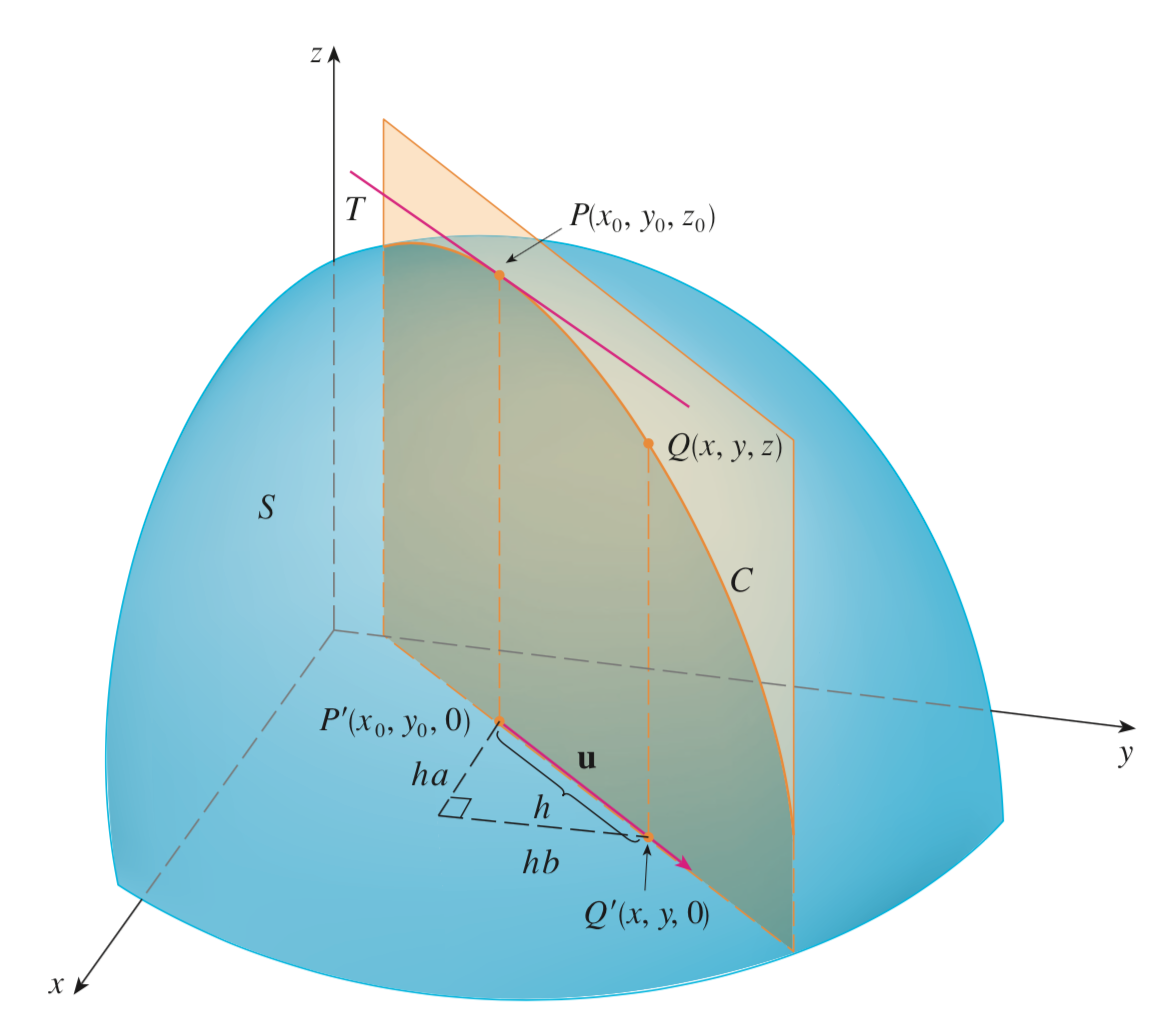
\includegraphics[width=0.6\textwidth]{./images/ch9/dd-1.png}
\end{center}
如图,所谓的方向导数可以理解为曲面$z=f(x,y)$与过$\bm{u}$的平面
的交线的切线关于$u$的斜率。也即: 
$$k=\lim\limits_{h\to 0}\df{z(Q)-z(P)}{h}$$

\begin{thx}
	{\bf $z=f(x,y)$在$(x_0,y_0)$沿$\bm{u}=(\cos\alpha,\cos\beta)$的方向导数:}
	$${D_uf(x_0,y_0)=\lim\limits_{h\to 0}
	\df{f(x_0+h\cos\alpha,y_0+h\cos\beta)-f(x_0,y_0)}{h}}$$
\end{thx}
方向导数也常常记为$\df{\p z}{\p u}$。显然,
$$D_if(x_0,y_0)=f\,'_x(x_0,y_0),
D_jf(x_0,y_0)=f\,'_y(x_0,y_0)$$

{\color{red} {\bf 注意:}同济教材上定义方向导数时,是令$t\to0^+$,而不是
$t\to0$。按照前一种定义,$z=\sqrt{x^2+y^2}$在原点处沿任意方向的方向
导数存在,但偏导不存在。按后一种定义,若某个函数沿任意方向的方向导数均存在,则
偏导数必存在。}

\begin{thx}
	{\bf 可微与方向导数的关系:}设函数$z=f(x,y)$在$P(x_0,y_0)$处可微, 
	则在该点处沿任意方向$\bm{u}$的方向导数存在, 且
	$$D_uf(x_0,y_0) =f\,'_x(x_0,y_0)\cos\alpha+f\,'_y(x_0,y_0)\cos\beta$$
	其中$\cos\alpha,\cos\beta$为$\bm{u}$的方向余弦。
\end{thx}

{\bf 例:}求函数$f(x,y)=xe^{2y}+\cos(xy)$在点$(1,0)$处沿
$\bm{u}=(3,-4)$的方向导数。

{\bf 例:}求函数$f(x,y,z)=x^2\cos y+e^{-y}\ln(x+z)$在点$(1,0,0)$处沿
$\bm{u}=3\bm{i}-4\bm{j}$的方向导数。

\subsection{梯度(向量)}

\begin{thx}
	{\bf 函数$z=f(x,y)$在$(x_0,y_0)$处的梯度:}
	$$\bigtriangledown
	f(x_0,y_0)=(f\,'_x(x_0,y_0),f\,'_y(x_0,y_0))=\bm{\mathrm{grad}}\,f$$
\end{thx}
前述可微与方向导数的关系可写为
$$D_uf=\bigtriangledown f\cdot\bm{e}_u,$$
根据向量点积的几何意义,可知方向导数也即梯度在给定方向上的投影长度。
同时,不难看出,沿着梯度方向行进,方向导数将取最大值。以爬山为例,
沿着梯度方向行进,坡度将是最大的,因此梯度方向通常被称为{\kaishu 最快上升方向}。

{\bf 例:}设某座山的表面对应于函数$z=15-3x^2-2y^2$,登山者站在其上的
$P(1,-2,4)$点,问其向哪个方向攀登坡度最陡?

{\bf 思考:}在画有等高线的地图上,如何判断何处最陡峭?(等高线最密集的方向!)

{\bf 梯度的几何意义:}$\bigtriangledown f$对应于$f(\bm{x})=c$的法线方向
\begin{center}
	\resizebox{!}{4.5cm}{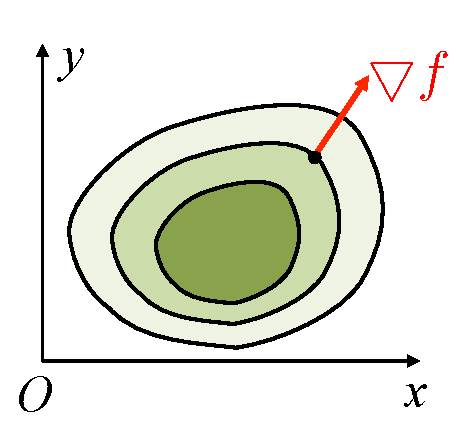
\includegraphics{./images/ch10/fxyc.pdf}}\hspace{3cm}
	\resizebox{!}{4.5cm}{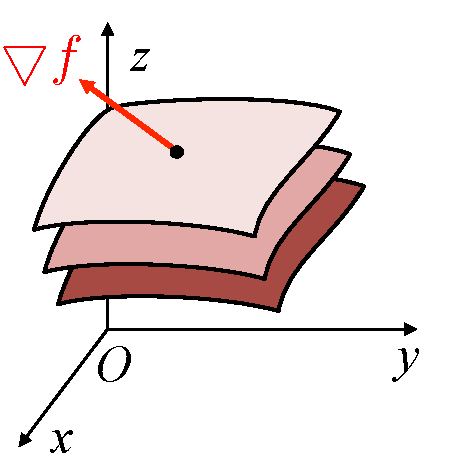
\includegraphics{./images/ch10/fxyzc.pdf}}
	
	等值(高)线:$f(x,y)=c$\hspace{3cm}等值面:$f(x,y,z)=c$
\end{center}

理解了梯度的几何意义,可以很容易地得到如下的定理,它是对一元函数的Fermat引理的推广。
\begin{thx}
	{\bf 可微多元函数极值的必要条件:}若$\bm{x}_0$为可微函数$f(\bm{x})$
	的一个{\it 局部最小(大)值}点,则对任意$\bm{u}\ne 0$,$D_{\bm{u}}
	f(\bm{x}_0)=0$。
\end{thx}

\begin{shaded}
	{\bf 向量场与势函数}
	
	如果对于空间区域$G$内的任一点$M$,都有一个确定的数量$f(M)$与之对应,则称在
	该空间区域内确定了一个{\it 数量场}(例如:{\it 温度场、密度场}等)。一个数量
	场可用一个数量函数$f(M)$来确定。
	
	与之类似,如果与点$M$对应的是一个向量$\bm{F}(M)$,则称在该空间区域内确定了
	一个{\it 向量场}(例如:{\it 引力场、速度场})。一个向量场可用一个向量值函数
	$\bm{F}(M)$来确定。
	
	若向量场$\bm{F}(M)$是某个数量函数$f(M)$的梯度(也即$\bigtriangledown
	f=\bm{F}$),则称$f(M)$是向量场$\bm{F}(M)$ 的一个{\it 势函数},称$\bm{F}(M)$为{\it
	势场}。由此可知,由数量函数$f(M)$ 产生的梯度场$\bigtriangledown f(M)$是一个势场。
	但需要注意,{\it 并非每个向量场都是势场。}
	
\end{shaded}

\subsection{Hessian矩阵}

\begin{thx}
	{\bf 多元函数的Hessian矩阵:}
	设$f(\bm{x})\,(\bm{x}=(x_1,x_2,\ldots,x_n))$的所有二阶偏导数连续,则 
	$$H=\left[\begin{array}{cccc}
		\df{\p^2 f}{\p x_1^2} & \df{\p^2 f}{\p x_1\p x_2} & \ldots & \df{\p^2
		f}{\p x_1\p x_n}\\[10pt]
		\df{\p^2 f}{\p x_2\p x_1} & \df{\p^2 f}{\p x_2^2} & \ldots & \df{\p^2
		f}{\p x_2\p x_n}\\[10pt]
		\ldots & \ldots & \ldots & \ldots\\[6pt]
		\df{\p^2 f}{\p x_n\p x_1} & \df{\p^2 f}{\p x_n\p x_2} & \ldots & \df{\p^2
		f}{\p x_n^2}
		\end{array}\right]
	=\bigtriangledown^2 f(\bm{x})$$
	称为其Hessian矩阵。
\end{thx}

{\bf 例:}计算$f(x,y)=x^4+xy+(1+y)^2$的Hessian矩阵。

{\bf 例:}设$\bm{a},\bm{b},\bm{x}\in\mathbb{R}^n,\bm{Q}
\in\mathbb{R}^{n\times n},\bm{Q}=\bm{Q}^T,c\in\mathbb{R}$,
求以下函数的梯度与Hessian矩阵:
\begin{enumerate}[(1)]
  \setlength{\itemindent}{1cm}
  \item $f(\bm{x})=\bm{b}\bm{x}^{T}+c$
  \item $g(\bm{x})=\df 12\bm{x}\bm{Q}\bm{x}^T+\bm{b}\bm{x}^{T}+c$
\end{enumerate}

\subsection{多元Taylor公式}

\begin{thx}
	{\bf 多元函数的Taylor公式:}设$n$元函数$f(\bm{x})$在$\bm{x}_0$的某邻域内二阶偏导数连续, 
	则:对该邻域内任意点$\bm{x}$, 存在$\theta\in(0,1)$, 使得
	\begin{eqnarray*}
		f(\bm{x}) & = & f(\bm{x}_0)+\bigtriangledown f(\bm{x}_0)(\bm{x}-\bm{x}_0)^T\\
		& & + \df 12(\bm{x}-\bm{x}_0)\bigtriangledown^2
		f(\bm{x}_0+\theta(\bm{x}-\bm{x}_0))(\bm{x}-\bm{x}_0)^T
	\end{eqnarray*}
	该公式称为{\bf $f(\bm{x})$在$\bm{x}_0$处带Lagrange余项的二阶Taylor公式} 
\end{thx}
类似地,有
\begin{thx}
	{\bf $f(\bm{x})$在$\bm{x}_0$处带Peano余项的Taylor公式:}
	\begin{eqnarray*}
		f(\bm{x}) & = & f(\bm{x}_0)+\bigtriangledown f(\bm{x}_0)(\bm{x}-\bm{x}_0)^T\\
		& & + \df 12(\bm{x}-\bm{x}_0)\bigtriangledown^2
		f(\bm{x}_0)(\bm{x}-\bm{x}_0)^T+\circ(|\bm{x}-\bm{x}_0|^2)
	\end{eqnarray*}
\end{thx}
与一元函数类似,Taylor公式中去掉余项的部分称为Taylor多项式。
不难验证,多元函数的二阶Taylor多项式和该函数在展开的点处是{\kaishu 二阶相切}的,也即
{\kaishu 二者的梯度向量和Hessian矩阵相同}。这个性质类似于一元函数的Taylor多项式的
定义,只是其中的一阶导数和二阶导数被替换成了多元函数的梯度和Hessian矩阵。

{\bf 例:}求$f(x,y)=x^4+xy+(1+y)^2$在原点处带Peano余项的一阶及二阶Taylor公式。

[提示]:$f(x,y)=1+2y+(xy+y^2)+\circ(x^2+y^2)$

不论是一元还是多元多项式函数,关于其Taylor展开都有如下的结论成立:
\begin{thx}
	{\bf 多项式函数的Taylor展开:}$n$次多项式的在给定点$x_0$处的$m$阶Taylor多项式,
	就是其关于$(x-x_0)$的$m$次截断多项式(即截取多项式中所有幂次不超过$m$的项所得到的
	多项式)。
\end{thx}

\begin{shaded}
	{\bf 二元函数$f(x,y)$在$(x_0,y_0)$处带Lagrange余项的的$n$阶Taylor公式}
	
	设$f(x,y)$在$(x_0,y_0)$附近存在$n+1$阶偏导数,则存在$\theta\in(0,1)$,使得
	\begin{align*}
		f(x+\Delta x,y+\Delta y)&=\sum\limits_{k=0}^n
		\df1{k!}\left(\Delta x\df{\p}{\p x}+\Delta y\df{\p}{\p y}\right)^kf(x_0,y_0)\\
		&+\df1{(n+1)!}\left(\Delta x\df{\p}{\p x}+\Delta y\df{\p}{\p y}\right)
		^{n+1}f(x_0+\theta\Delta x,y_0+\theta\Delta y)
	\end{align*}
	其中
	$$\left(\Delta x\df{\p}{\p x}+\Delta y\df{\p}{\p y}\right)^kf(x_0,y_0)
	=\sum\limits_{p=0}^k\mathrm{C}_k^p\Delta x^p\Delta y^{k-p}
	\left.\df{\p^kf}{\p x^p\p y^{k-p}}\right|_{(x_0,y_0)}$$
	
	若记$\bigtriangledown=\left(\df{\p}{\p x},\df{\p}{\p y}\right)$,
	$\bm{x}=(x,y),\Delta\bm{x}=(\Delta x,\Delta y)$,则以上公式也可以表示为
	$$f(\bm{x}+\Delta\bm{x})=\sum\limits_{k=0}^n
	\df1{k!}\left(\Delta\bm{x}
	\cdot\bigtriangledown\right)^kf(\bm{x}_0)+\df1{(n+1)!}
	\left(\Delta\bm{x}\cdot\bigtriangledown\right)^{n+1}f(
	\bm{x}+\theta\Delta\bm{x})$$
	这种记号显然更加有利于将Taylor公式推广到更多元的函数情形。
	
	{\bf 例:}函数$f(x,y)=\ln(1+x+y)$在$(0,0)$处带Lagrange余项的三阶Taylor公式
	
	[解]:
	$$f'_x(x,y)=f'_y(x,y)=\df1{1+x+y}$$
	$$f''_{xx}(x,y)=f''_{xy}(x,y)=f''_{yy}(x,y)=-\df1{(1+x+y)^2},$$
	$$\df{\p^3f}{\p x^p\p y^{3-p}}=\df{2!}{(1+x+y)^3},\;p=0,1,2,3,$$
	$$\df{\p^4f}{\p x^p\p y^{4-p}}=-\df{3!}{(1+x+y)^4},\;p=0,1,2,3,4,$$
	故
	\begin{align*}
		\left(\Delta x\df{\p}{\p x}+\Delta y\df{\p}{\p y}\right)f(0,0)
		&=\Delta xf'_x(0,0)+\Delta yf'_y(0,0)
		=\Delta x+\Delta y,\\
		\left(\Delta x\df{\p}{\p x}+\Delta y\df{\p}{\p y}\right)^2f(0,0)
		&=\Delta x^2f''_{xx}(0,0)+2\Delta x\Delta yf''_{x,y}(0,0)
		+\Delta y^2f''_{yy}(0,0)\\
		&=-(\Delta x+\Delta y)^2,\\
		\left(\Delta x\df{\p}{\p x}+\Delta y\df{\p}{\p y}\right)^3f(0,0)
		&=\Delta x^3f'''_{xxx}(0,0)+3\Delta x^2\Delta yf'''_{xxy}(0,0)\\
		&\quad +3\Delta x\Delta y^2f'''_{xyy}(0,0)+\Delta y^3f'''_{yyy}(0,0)\\
		&=2(\Delta x+\Delta y)^3
	\end{align*}
	综上,存在$\theta\in(0,1)$,使得
	$$\ln(1+x+y)=x+y-\df12(x+y)^2+\df13(x+y)^3-\df14\df{(x+y)^3}
	{(1+\theta x+\theta y)^4}$$
\end{shaded}

% {\bf 例:}设函数$f(x,y)$二阶偏导函数处处连续,且$f(0,0)=0$,
% $$|f'_x(x,y)|\leq 2|x-y|,\quad |f'(x,y)|\leq2|x-y|,$$
% 证明:$|f(5,4)|\leq 1$。

\begin{ext}
	{\bf 课后作业}
	\begin{enumerate}
	  \item 求曲面$z=x^2+y^2$上的点$(1,1,2)$处沿椭圆$\df{x^2}{8}+\df{y^2}{2}=1$
	  在$(2,1)$的外法向的方向导数。
	  \item 试证曲面$\sqrt{x}+\sqrt y+\sqrt z=\sqrt a\,(a>0)$
	  在任一点处的切平面在三个坐标轴上的截距之和为常数。
	  \item 已知曲面方程$z=xe^{y/x}$,证明:曲面上任一点$M$处的法线与其
	  向径垂直。
	  \item 求函数$xe^{x+y}$在原点处带Peano余项的二阶Taylor公式。
	\end{enumerate}
\end{ext}

\section{多元函数的极值与条件极值}

{\kaishu 极值}也即局部唯一的最值。
\begin{thx}
	{\bf $n$元函数$f(\bm{x})$在$\bm{x}_0$处取极小值:}
	$f(\bm{x}_0)$有定义,且对$\bm{x}_0$某去心邻域内的任意点
	$\bm{x}$,恒有$f(\bm{x})>f(\bm{x}_0)$
\end{thx}

{\bf 例:}判断$(1,\pm1)$是否为$f(x,y)=(y-x^2)(y-x^4)$的极值点,若是,
是极大值点还是极小值点。

[解]:如图,
\begin{center}
	\resizebox{!}{4cm}{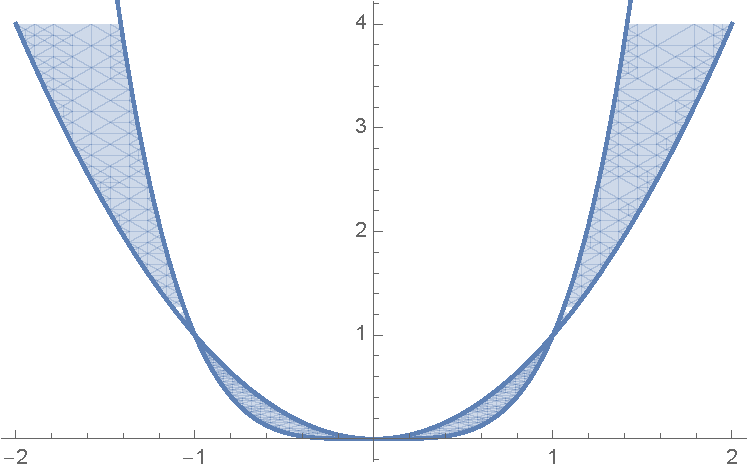
\includegraphics{./images/ch10/yx2yx4.pdf}}
\end{center}
$(\pm1,1)$恰为曲线$y=x^2$和$y=x^4$的交点,且$f(\pm1,1)=0$。注意到,在图中
的阴影区域$f(x,y)\leq0$,在阴影之外的区域$f(x,y)\geq0$,故可知$(\pm1,1)$附近
的取值均是有正有负的,所以它们不可能是$f(x,y)$的极值点。\fin

\subsection{极值的判定}

在极值可能的位置上,一元函数和多元函数具有相似的性质:
\begin{itemize}
  \item 一元函数的极值点可能为{\kaishu 驻点、边界点或不可导点 }
  \item 二元函数的极值点可能为{\kaishu (二维)驻点、边界或不可微点} 
\end{itemize}

以下定理是对一元函数Fermat引理的推广
\begin{thx}
	{\bf 可微函数极值点的必要条件:}若可微函数$f(\bm{x})$在$\bm{x}_0$处取极值,则$\bm{x}_0$
	为$f(\bm{x})$的{\bf 驻点},即:$\bigtriangledown f(\bm{x}_0)=0$
\end{thx}
由此立即可以得到如下的推论
\begin{thx}
	若$f(\bm{x})$在$\bm{x}_0$处偏导连续且取极值,则对应曲面
	在该点处有水平切面。
\end{thx}

\begin{shaded}
	{\bf 二元函数的驻点与极值点}
	\begin{center}
		\resizebox{!}{4.5cm}{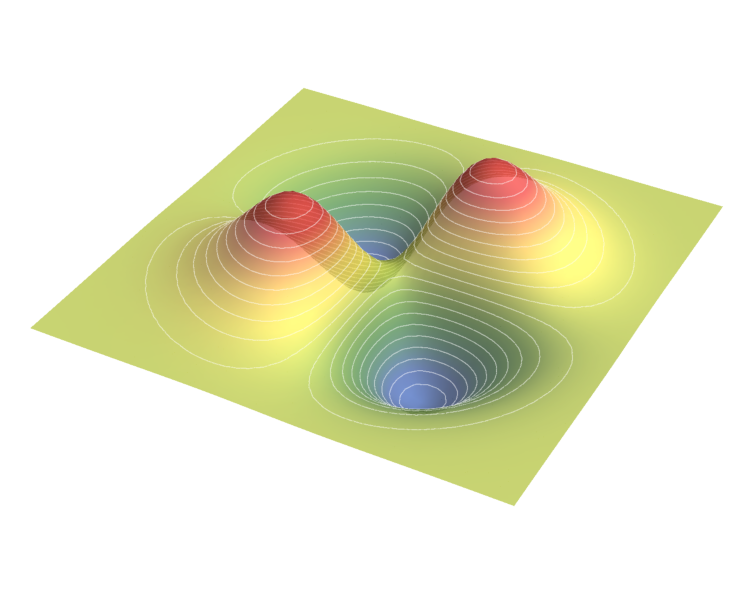
\includegraphics{./images/ch10/3DLim-1-1.pdf}}\quad
		\resizebox{!}{4.5cm}{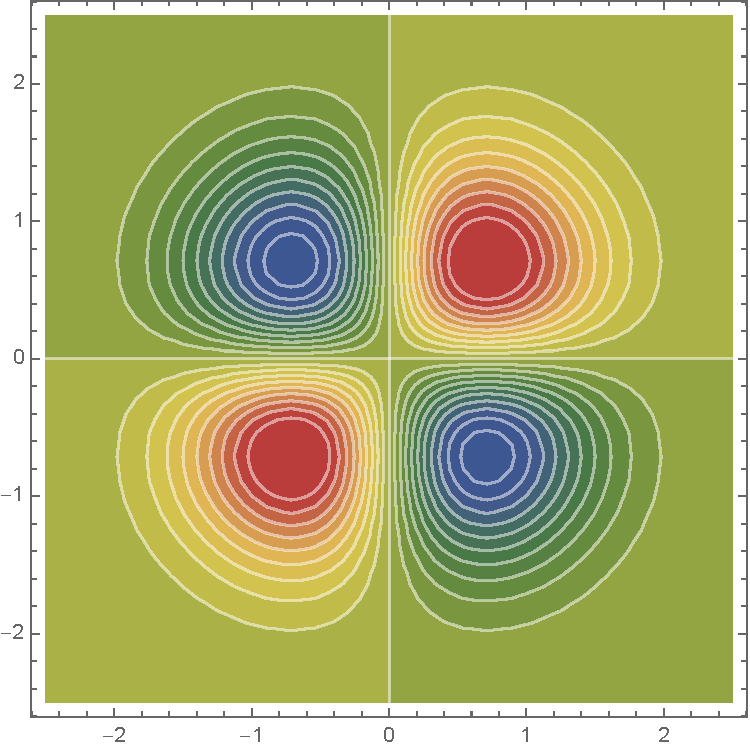
\includegraphics{./images/ch10/3DLim-1-2.pdf}}
		
		{\it 可微函数的极值点必为驻点}
		\bs
		
		\resizebox{!}{4.5cm}{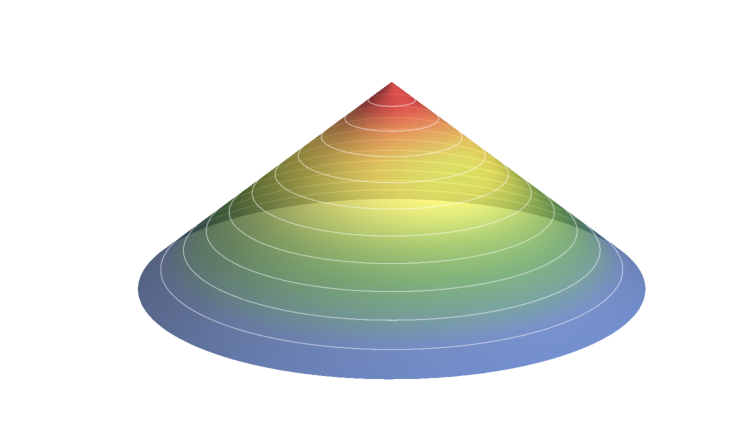
\includegraphics{./images/ch10/3DLim-3-1.pdf}}\quad
		\resizebox{!}{4.5cm}{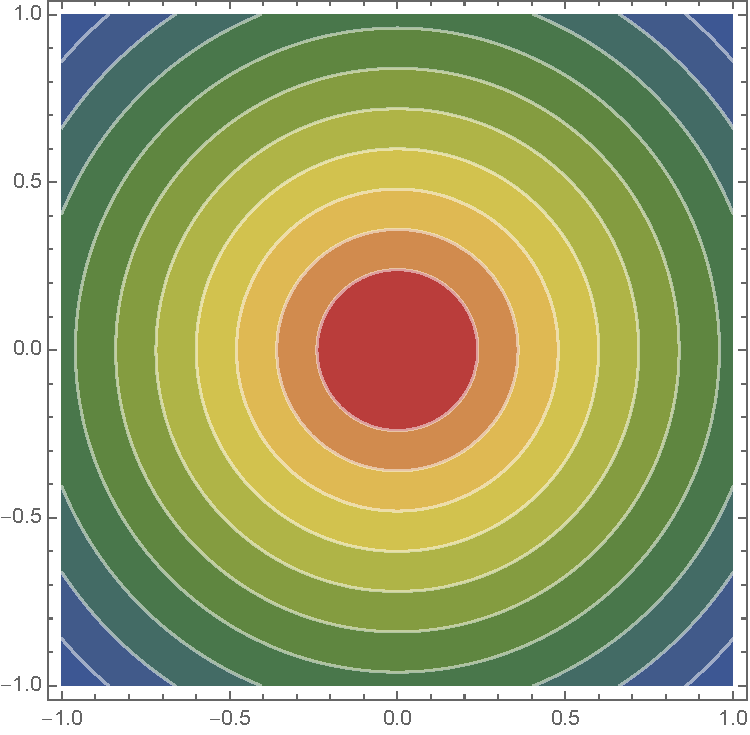
\includegraphics{./images/ch10/3DLim-3-2.pdf}}
		
		{\it 极值点未必是驻点}
		\bs
		
		\resizebox{!}{4.5cm}{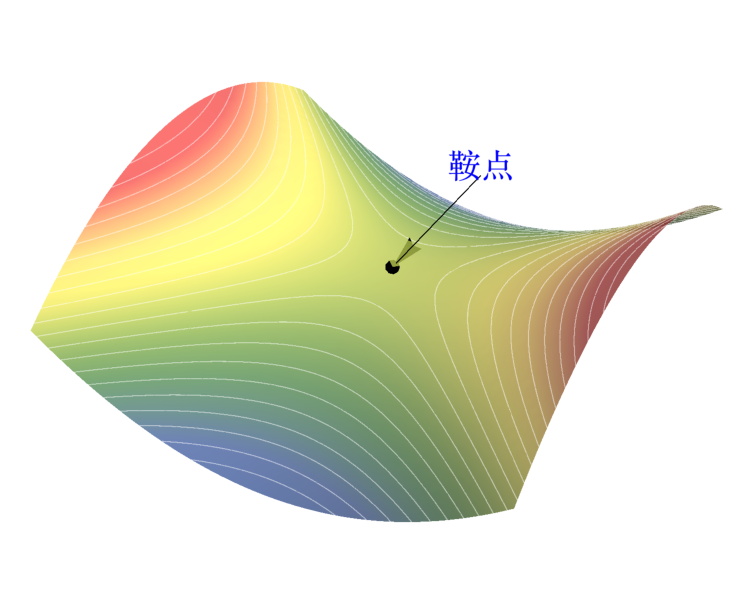
\includegraphics{./images/ch10/3DLim-2-1.pdf}}\quad
		\resizebox{!}{4.5cm}{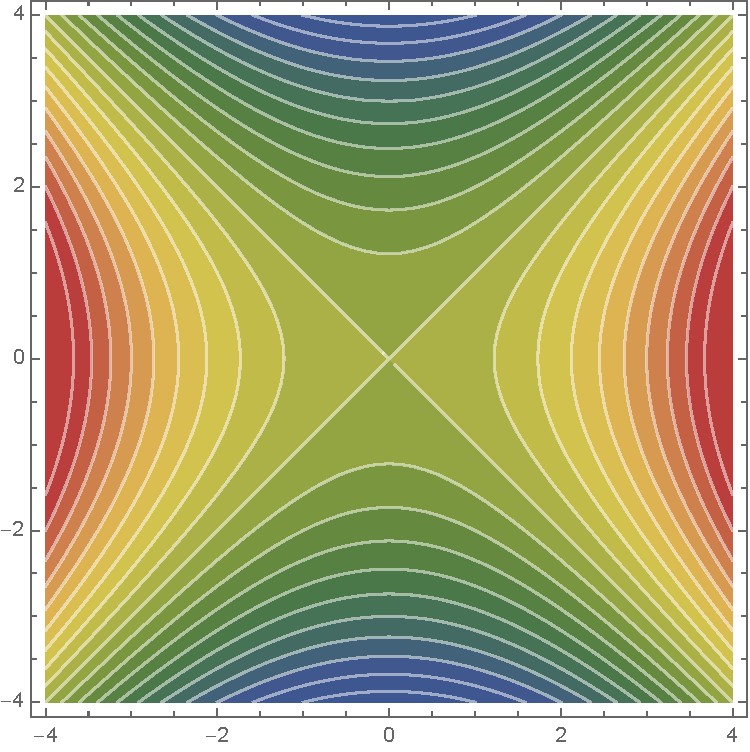
\includegraphics{./images/ch10/3DLim-2-2.pdf}}
		
		{\it 驻点未必是极值点}
	\end{center}
\end{shaded}

\begin{thx}
	{\bf 多元函数极值的充分条件:}设$f(\bm{x})$在$\bm{x}_0$处存在二阶连续偏导数,
	$\bigtriangledown f(\bm{x}_0)=0$,则由
	$\bigtriangledown^2 f(\bm{x}_0)$正定、负定和不定
	可分别判定$\bm{x}_0$为$f(\bm{x})$的极小值、极大值和鞍点。
\end{thx}
由此不难发现,对多元函数而言,$\bigtriangledown f$和$\bigtriangledown^2 f$
在几何性质上类似于一元函数的一阶和二阶导数。
\begin{thx}
	{\bf 二元函数极值的充分条件:}$f(x,y)$在$(x_0,y_0)$二阶偏导数连续,$\bigtriangledown f(x_0,y_0)=0$,
	记$A=f\,''_{xx}(x_0,y_0),\,B=f\,''_{xy}(x_0,y_0),\,C=f\,''_{yy}(x_0,y_0)$,则
	\begin{enumerate}%[(1)]
% 	  \setlength{\itemindent}{1cm}
	  \item 若$A>0$且$AC-B^2>0$,$(x_0,y_0)$为$f(x,y)$的极小值点;
	  \item 若$A<0$且$AC-B^2>0$,$(x_0,y_0)$为$f(x,y)$的极大值点;
	  \item $AC-B^2<0$,$(x_0,y_0)$为$f(x,y)$的鞍点。
	\end{enumerate}
\end{thx}

{\bf 例:}求$z=-xye^{-(x^2+y^2)}$的极值。

极值的判定问题往往比最值的判定更加困难,对于多元函数更是如此。

{\bf 例:}已知$\lim\limits_{(x,y)\to(0,0)}\df{f(x,y)-xy}{3x^2+2y^2}=1$,
判断$(0,0)$是否为$f(x,y)$的极值点,若是,是极大值还是极小值?

[解]:由已知极限可得
$$\lim\limits_{(x,y)\to(0,0)}\df{f(x,y)-xy-3x^2-2y^2}{3x^2+2y^2}=0,$$
从而
$$f(x,y)=3x^2+2y^2+xy+\circ(3x^2+2y^2),$$
又由于
$$\df{\circ(3x^2+2y^2)}{3x^2+2y^2}\leq\df{\circ(3x^2+2y^2)}{x^2+y^2}
\leq\df{\circ(3x^2+2y^2)}{x^2+2/3y^2},$$
由夹逼定理可知:
$$\lim\limits_{(x,y)\to(0,0)}\df{\circ(3x^2+2y^2)}{x^2+y^2}=0,$$
故
$$f(x,y)=3x^2+2y^2+xy+\circ(x^2+y^2).$$
该式可视为$f(x,y)$在$(0,0)$处的Taylor展开,从而可知
$$f''_{xx}(0,0)=3,\quad f''_{yy}(0,0)=2,
\quad f''_{xy}(0,0)=f''_{yx}(0,0)=1/2,$$
于是
$$\bigtriangledown^2f(0,0)=\left[\begin{array}{cc}
f''_{xx}(0,0) & f''_{xy}(0,0) \\ f''_{yx}(0,0) & f''_{yy}(0,0)
\end{array}\right]
=\left[\begin{array}{cc}
3 & 1/2 \\ 1/2 &2
\end{array}\right],$$
这是一个正定矩阵,由可微函数极值的充分条件,可知$(0,0)$为$f(x,y)$的极小值点。
\fin

\subsection{条件极值}

{\bf 例:}求函数$z=\sqrt{4-x^2-y^2}$的满足$(x-1)^2+y^2=1$的极值点。

\begin{center}
	\resizebox{!}{4cm}{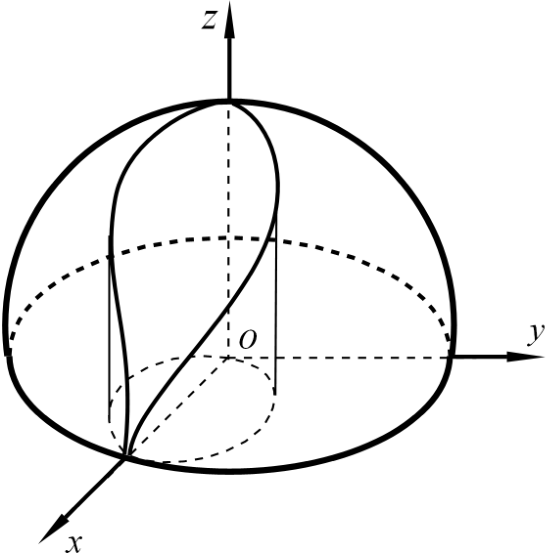
\includegraphics{./images/ch10/viviani.pdf}} 
\end{center}

{\bf 例:}求以$(0,0),(0,1),(1,0)$为顶点的三角形区域内
到该三点距离平方和最大的点。

通过这个例子可以看到,在一个看似一般的多元函数极值问题中,边界上的情况往往更不好处理。
特别是考虑到一些边界的特殊性,可能导致问题变得特别复杂,为此,有必要考虑引入一种
特定的方法专门解决这类问题,也即所谓的{\kaishu 条件极值问题}。

\begin{thx}
	{\bf 条件极值问题}:在满足一定条件$g(\bm{x})=0$(可以包含多个方程)
	的前提下,求多元函数$z=f(\bm{x})$极值,一般也表述为:
	{\kaishu 求$f(\bm{x})$满足$g(\bm{x})=0$的极值},其中,
	$g(\bm{x})=0$称为{\kaishu 约束条件},$f(\bm{x})$称为{\kaishu 目标函数}。
\end{thx}

对于条件极值问题,可以采用一种统一的方法来进行求解:

\begin{thx}
	{\bf Lagrange乘子法:}考虑$f(x,y)$满足$g(x,y)=0$的极值问题,构造
	{\bf Lagrange辅助函数}
	$${L(x,y,\lambda)=f(x,y)+\lambda g(x,y)},$$
	则
	\begin{enumerate}%[(1)]
% 	  \setlength{\itemindent}{1cm}
	  \item $L(x,y,\lambda)$的极值点即为所求条件极值的极值点; 
	  \item $L(x,y,\lambda)$的极值点$(x_0,y_0,\lambda_0)$必满足 
	  $\bigtriangledown L(x_0,y_0,\lambda_0)=0.$
	\end{enumerate}
\end{thx}

几何上,Lagrange乘子法的意义参见下图:
\begin{center}
	\resizebox{!}{4.5cm}{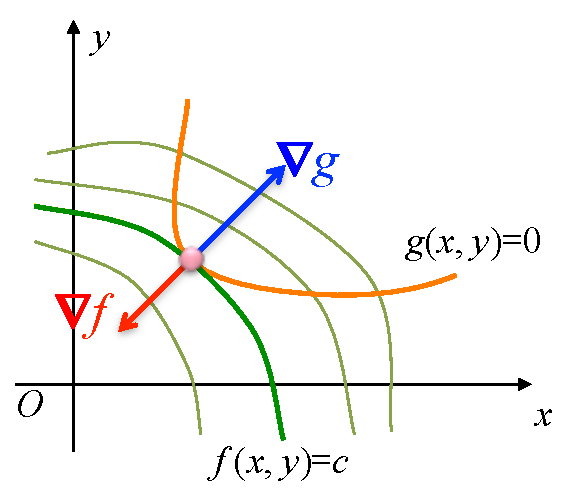
\includegraphics{./images/ch10/reshill.pdf}} 
\end{center}
若$f(x,y)=c$和$g(x,y)=0$光滑,则在极值点处必有
$${\bigtriangledown f // \bigtriangledown g}$$
即存在$\lambda_0$,使得
$$
{\left\{\begin{array}{l}
	f\,'_x(x_0,y_0)=\lambda_0g\,'_x(x_0,y_0)\\
	f\,'_y(x_0,y_0)=\lambda_0g\,'_y(x_0,y_0)
\end{array}
\right.}$$

Lagrange乘子法的最大优点是使我们能够在不必过度关注约束条件结构的情况下求解
条件极值问题。

{\bf 例:}求函数$z=\sqrt{4-x^2-y^2}$的满足$(x-1)^2+y^2=1$的极值点。
\begin{center}
	\resizebox{!}{6cm}{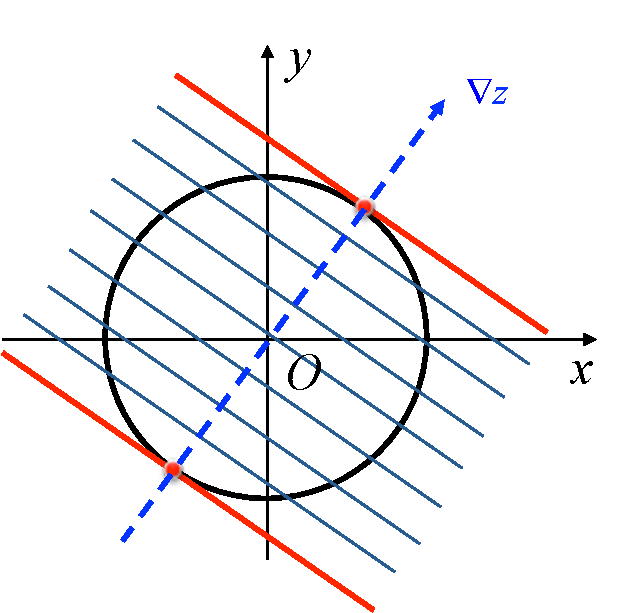
\includegraphics{./images/ch10/lagxy.pdf}}
\end{center}

根据条件极值问题形式的不同,Lagrange乘子法也可以有相应的形式,诸如:
\begin{enumerate}[(1)]
  \setlength{\itemindent}{1cm}
  \item 更高维度(更多变量)的问题,例如:求函数$w=f(x,y,z)$满足$g(x,y,z)=0$的极值; 
  
  [思路]:记$L=f(x,y,z)+\lambda g(x,y,z)$,令$\bigtriangledown L=0$ 
  \item 更多约束(约束条件)的问题,例如:求函数$w=f(x,y,z)$满足$g_1(x,y,z)=g_2(x,y,z)=0$的极值 
  
  [思路]: 记
  $$L=f(x,y,z)+\lambda_1 g_1(x,y,z)+\lambda_2 g_2(x,y,z),$$
  令$\bigtriangledown L=0$
\end{enumerate}

{\bf 例:}求平面$x+y+z=1$与柱面$x^2+y^2=1$上距离原点最近和最远的点。
\begin{center}
	\resizebox{!}{5cm}{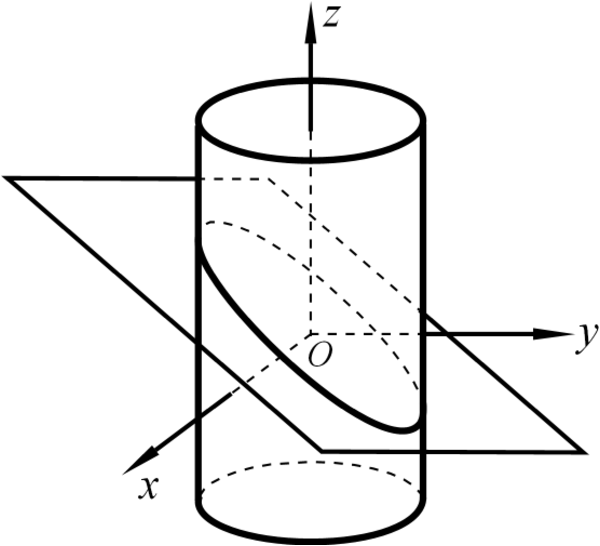
\includegraphics{./images/ch10/planeCy.pdf}}
\end{center}

{\bf 例:}要制作一个表面积为$a^2$的无盖长方体盒子,
问其长宽高各为多少时,盒子的容积最大。

[提示]:$x=y=\df a{\sqrt 3},\;z=\df a{2\sqrt3}$,$V_{\max}=\df{a^2}{6\sqrt 3}$。

{\bf 例:}当$x,y,z$均大于零时,求函数$u=\ln x+2\ln y+3\ln z$
在球面$x^2+y^2+z^2=6R^2$上的最大值,并证明对任意正数
$a,b,c$,成立不等式
$$ab^2c^3\leq 108\left(\df{a+b+c}{6}\right)^6$$

[解]:由Lagrange乘子法,记
$$L=xy^2z^3+\lambda(x^2+y^2+z^2-6R^2),$$
令$\bigtriangledown L=0$,可解得$x=R,y=\sqrt2 R,z=\sqrt3 R$,从而有:
$$xy^2z^3\leq 6\sqrt 3R^6=6\sqrt 3\left(\df{x^2+y^2+z^2}{6}\right)^3.$$
也即
$$x^2y^4z^6\leq 108\left(\df{x^2+y^2+z^2}{6}\right)^6.$$
记$a=x^2,b=y^2,c=z^2$,即证。\fin

[提示]:使用Lagrange乘子法求解该题有不小的计算量,事实上,也可以直接使用平均值不等式
的方法来求解。

注意到$a,b,c>0$时
$$\df{a+b+c}6=\df16\left(a+\df b2+\df b2+\df c3+\df c3+\df c3\right)
\geq \sqrt[6]{\df{ab^2c^3}{108}},$$
稍加整理即为第二问的不等式(当且仅当$a=\df b2=\df c3$时,等号成立)。

记$a=x^2,b=y^2,c=z^2$,则由上式,当$x^2+y^2+z^2=6R^2$时,有
$$x^2y^4z^6\leq108\left(\df{x^2+y^2+z^2}{6}\right)^6
=108\left(R^2\right)^6$$
进而\ps{\b 求解极值和条件极值问题,不应拘泥于Lagrange乘子法的“套路”,合理地
使用已经熟悉的不等式,常常能够使计算大为简化}
$$xy^2z^3\leq6\sqrt3R^6.$$
并且,我们容易知道当且仅当$x^2=\df{y^2}2=\df{z^2}3$时,取到以上的最大值。

{\bf 例:}在半径为$R$的圆的内接三角形中,求面积最大者。

[提示]:圆的内接三角形的面积由圆的半径$r$和各边对应的圆心角$\alpha,\beta,\gamma$
确定,具体地
$$S=\df{r^2}2(\sin\alpha+\sin\beta+\sin\gamma),\quad
(\alpha+\beta+\gamma=2\pi)$$
如果不使用Lagrange乘子法,利用变量替换$\gamma=2\pi-\alpha-\beta$,则
\begin{align*}
	\sin\alpha+\sin\beta+\sin\gamma
	&=2\sin\df{\alpha+\beta}2\cos\df{\alpha-\beta}2-\sin(\alpha+\beta)\\
	&=2\sin\df{\alpha+\beta}2\cos\df{\alpha-\beta}2-2\sin\df{\alpha+\beta}2
	\cos\df{\alpha+\beta}2\\
	&=2\sin\df{\alpha+\beta}2\left(\cos\df{\alpha-\beta}2
	-\cos\df{\alpha+\beta}2\right)\\
	&=4\sin\df{\alpha+\beta}2\sin\df{\alpha}2\sin\df{\beta}2
	\quad(0\leq\alpha+\beta\leq2\pi)
\end{align*}
这样问题就转换成了求解二元函数$\sin\df{\alpha+\beta}2\sin\df{\alpha}2\sin\df{\beta}2$
在闭区域$0\leq\alpha+\beta\leq2\pi$上的极值问题,接下来还会有相当大的计算量。

如果使用Lagrange乘子法,则可设\ps{\b 这个例子说明,使用Lagrange乘子法,并不一定总是
计算量很大,所以我们应该尽可能考虑综合使用各种可行的方法}
$$L=\sin\alpha+\sin\beta+\sin\gamma+\lambda(\alpha+\beta+\gamma-2\pi),$$
于是$\bigtriangledown L=0$也即
$$
	\left\{\begin{array}{l}
		\cos\alpha+\lambda=0\\
		\cos\beta+\lambda=0\\
		\cos\gamma+\lambda=0\\
		\alpha+\beta+\gamma-2\pi=0
	\end{array}\right.
$$
观察方程组的特点,容易发现$\alpha=\beta=\gamma$时取极值,计算量较前面的方法大为减少。

{\bf 例:}设$F(x,y,z)$在条件$\varphi(x,y,z)=0$和$\psi(x,y,z)=0$
之下在点$P_0(x_0,y_0,z_0)$处取得极值$m$,证明:曲面
$F(x,y,z)=m,\varphi(x,y,z)=0$和$\psi(x,y,z)=0$
在$P_0$的法线共面,其中函数$F,\varphi,\psi$均有连续且不同时
为零的一阶偏导数。

{\bf 例:}现有资金$36$元,要建造一个无盖的长方体容器,已知底面造价为$3$元每平方米,
侧面造价为$1$元每平方米,求可造出的长方体的最大容积。

{\bf 例:}求函数$z=x^2-xy+y^2$在区域$D:|x|+|y|\leq 1$
上的最大和最小值。

[提示]:令$x+y=X,x-y=Y$,则\ps{任意形如$ax^2+bxy+cy^2$的函数都可以通过
该线性变换化为形如$AX^2+BY^2$的形式!}
$$z=x^2-xy+y^2=\df14X^2+\df34Y^2,$$
$$D:|x|+|y|\leq 1\quad\Leftrightarrow\quad |X|\leq1,|Y|\leq1$$
易知$|X|=|Y|=1$时,$z$取最大值$1$,$|X|=|Y|=0$时,$z$取最大值$0$.

如果使用普通的方法,计算量会大很多。

{\bf 例:}证明:函数$f(x,y)=e^{\cos x}-y^2$在全平面上有无穷多个极大值,但无极小值。

[提示]:如图\ps{对可微的一元函数而言,两个极大值点之间必有至少一个极小值点,对多元函数则不然!}
\begin{center}
	\resizebox{!}{5cm}{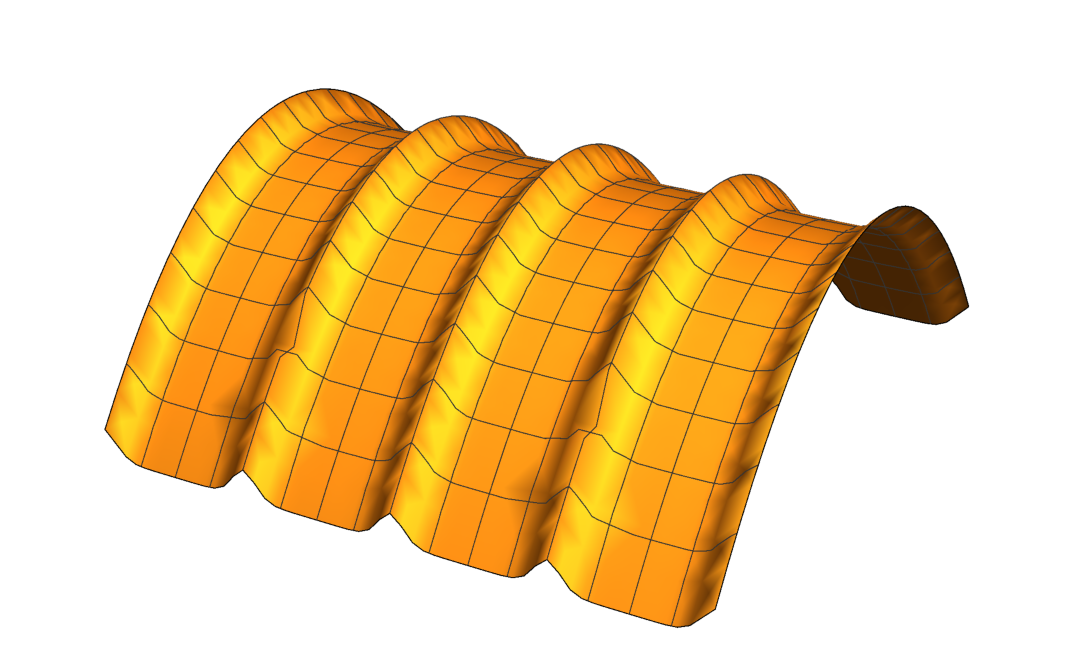
\includegraphics{./images/ch10/iUnD.pdf}}
\end{center}

\begin{ext}
	{\bf 课后作业}
	\begin{enumerate}
	  \item 求内接于椭球面$\df{x^2}{a^2}+\df{y^2}{b^2}+\df{z^2}{c^2}=1$
	  的长方体的最大体积。
	  \item 某公司的产品广告有电台和报纸两种发布途径,经研究发现,产品销售收入$U$(万元)与
	  投入的电台广告费用$T$(万元)和投入的报纸广告费用$P$(万元)满足如下关系
	  $$U=15+14T+32P-8TP-2T^2-10X^2.$$
	  \begin{enumerate}[(1)]
	    \item 在广告预算不封顶的情况下,求公司的最优广告策略;
	    \item 若广告总预算上限为$1.5$万元,求公司的最优广告策略。
	  \end{enumerate}
	  \item 已知$\lim\limits_{(x,y)\to(0,0)}\df{f(x,y)-4xy}{x^2+y^2}=1$,
	  判断$(0,0)$是否为$f(x,y)$的极值点,若是,是极大值还是极小值?
	\end{enumerate}
\end{ext}

\section{小结}

多元函数微分学是对一元函数微分学的推广,通过本章的学习,应该会对此留下比较深刻的印象。

然而,与从一元函数推广到向量值函数时的那种“轻松自如”不同,从一元到多元的推广显然要
复杂得多。在本章的学习中要特别注意把握两者的异同。

不同的地方,主要源自两个方面,一是从一维集合上升到二维集合,导致极限概念在理解上的差异
(从数学形式上看没有什么不同),二是从导数概念简单形式推广中遇到的问题(向量不能作分母),
导致在可导、可微概念上出现了诸多的差异。可以说,从一元微分学到多元微分学,一直是有异
有同相互交织的,能够在相互比照,理解推广的原理的同时,准确把握前后的差异,是深刻理解
本章所有结论的根本。

\begin{enumerate}
  \item {\bf 极限与连续}
  \begin{enumerate}[(1)]
    \item 二重极限存在性的判定
    \begin{itemize}
      \item {\it 套路1}:累次极限不同,则二重极限不存在
      \item {\it 套路2}:令$y=kx$,若相应的极限与$k$有关,则二重极限不存在
      \ps{\b 与$k$无关并不能说明二重极限存在!}
      \item {\it 套路3}:令$x=\rho\cos\theta,y=\rho\sin\theta$,则
      $(x,y)\to(x_0,y_0)\Leftrightarrow\rho\to0^+$,若极限
      $$\lim\limits_{\rho\to0^+}f(\rho\cos\theta(\rho),\rho\sin\theta(\rho))$$
      为常数,则二重极限存在。\ps{\b $\theta(\rho)$表示$\theta$的取值可能是与$\rho$有关的!}
%       二重极限与累次极限的关系:
%       $\lim\limits_{(x,y)\to(x_0,y_0)}f(x,y)=a\Rightarrow
%       \lim\limits_{x\to x_0}\lim\limits_{y\to y_0}f(x,y)=
%       \lim\limits_{y\to y_0}\lim\limits_{x\to x_0}f(x,y)=a$,反之不然!
%       \item 判定二重极限不存在:选择不同的路径,证明相应的极限不存在,即:若
%       对过$(x_0,y_0)$不同的连续曲线$y=y(x,k)$(例如$y=kx$),
%       $$\lim\limits_{x\to x_0\atop y=y(x,k)}f(x,y)=a(k)$$
%       不为常数,则二重极限不存在
%       \item 判定二重极限存在:利用极坐标变换,将$(x,y)\to(x_0,y_0)$转换为$\rho\to0^+$,
%       证明极限
%       $$\lim\limits_{\rho\to0^+}f(\rho\cos\theta(\rho),\rho\sin\theta(\rho))$$
%       为常数。
      
%       注意:{\it $\theta(\rho)$表示$\theta$的取值可能是与$\rho$有关的!}
      \item 重点掌握教材10.2节的例3-例5
      \item 注意各种不同极限形式的正确书写方法,例如
      $$\lim\limits_{(x,y)\to(x_0,y_0)}f(x,y)\quad
      \lim\limits_{x\to x_0\atop y\to y_0}f(x,y),\quad
      \lim\limits_{x\to x_0}\lim\limits_{y\to y_0}f(x,y),\quad
      \lim\limits_{x\to x_0\atop y=kx}f(x,y),\quad
      \lim\limits_{x\to x_0\atop y=0}f(x,y)
      $$
    \end{itemize}
    \item 连续与可微
    \begin{itemize}
      \item 有界闭区域上的多元连续函数与有界闭区间上的一元连续函数具有类似的性质:
      有界性、最值存在性和介值性
      \item 可微必连续,且偏导数存在
      \item 用定义证明$z=f(x,y)$在$(x_0,y_0)$可微:令$A=f'_x(x_0,y_0),B=f'_y(x_0,y_0)$,
      证明
      $$\lim\limits_{(0,0)\to(x_0,y_0)}
      \df{f(x_0+\Delta x,y_0+\Delta y)-f(x_0,y_0)
      -A\Delta x-B\Delta
      y}{\sqrt{(\Delta x)^2+(\Delta y)^2}}=0$$
      即可
      \item 重点掌握教材习题10.2节的16-17.
    \end{itemize}
  \end{enumerate}
  \item {\bf 偏导数、全微分与方向导数}
  \begin{enumerate}[(1)]
    \item 偏导数及其计算
    \begin{itemize}
      \item 偏导数的定义:除求导变量外,将其他自变量均视为常数(因此在实际计算某个
      点处的偏导时,可以先带入其他自变量的值)然后求导,例如
      $$\left.\df{\p}{\p x}(1+x+\arctan(xy))\right|_{(2,0)}=
      \left.\df{\d}{\d x}(1+x)\right|_{x=2}=1$$
      \item 偏导数的几何意义:$f'_x(x_0,y_0)$表示曲线$\left\{\begin{array}{l}
      z=f(x,y)\\ y=y_0
      \end{array}\right.$在$(x_0,y_0)$处的切线斜率,也相当于在该点处沿$\bm{i}$方向
      的方向导数$D_if(x_0,y_0)$
      \item 复合函数的偏导数:设$z=f(u,v),u=u(x,y),v=v(x,y)$,则
      $$z'_x=z'_uu'_x+z'_vv'_x$$
      {\it 链式法则:}画出变量之间的依赖关系图(树),标记出每条路线上对应的偏导数,
      按照“并联对应加法,串联对应乘法”的规则,综合写出所有可能的路径
      \item 隐函数求导:(1)确定那些变量是自变量,那些是因变量;(2)对所有给定的方程
      两边求(偏)导,解出相应的(偏)导数值;或者(2')对所有方程求全微分,解出所有因变量
      的全微分,然后根据一阶微分的形式不变性,确定相应的(偏)导数
    \end{itemize}
    \item 全微分:设$z=f(x,y)$,则
    $$\d z=f'_x\d x+f'_y\d y=\bigtriangledown f\cdot \d\bm{r},$$
    其中$\d\bm{r}=(\d x,\d y)$
    \begin{itemize}
      \item 全微分的应用:误差估计、判断不同参数(的误差)对测量值(的误差)的影响
    \end{itemize}
    \item 方向导数与梯度
    \begin{itemize}
      \item 方向导数的定义(以二元函数为例)
      $$\left.\df{\p f}{\p u}\right|_{(x_0,y_0)}=D_uf(x_0,y_0)
      =\lim\limits_{h\to0}\df{f(x_0+h\cos\theta,y_0+h\sin\theta)-
      f(x_0,y_0)}{h}$$
      其中$\bm{u}=|\bm{u}|(\cos\theta,\sin\theta)$
      \item 若$z=f(x,y)$可微,则沿任意方向的方向导数存在,且
      $$D_uf=\bigtriangledown f\cdot\bm{e}_u=\left(\bigtriangledown f\right)_u$$
      \begin{itemize}
        \item 推论1:沿梯度方向的方向导数值最大
        \item 推论2:梯度方向是该点处的最快上升方向
        \item 推论3:梯度方向垂直与该点处的等高线,且指向函数值增大的方向,例:
        (1)球面的{\it 外法向}为指向球外部的矢径方向
        (2)曲面$F(x,y,z)=0$可视为函数$w=F(x,y,z)$的一个等值面,故其法向量为 
        $\bigtriangledown F$
      \end{itemize}
    \end{itemize}
  \end{enumerate}
  \item {\bf 多元函数微分学的应用}
  \begin{enumerate}[(1)]
    \item 注意:
    \begin{itemize}
      \item 与一元函数相关概念的对应关系:梯度$\bigtriangledown f\leftrightarrow$一阶导数$f'$,
      Hessian矩阵$\bigtriangledown^2f\leftrightarrow$二阶导数$f''$
      \item 与一元函数相关方法的异同 
    \end{itemize}
    \item Taylor公式(以二元函数为例):$z=f(x,y)$在$(x_0,y_0)$处带Peano余项的二阶Taylor公式
      \begin{eqnarray*}
      f(x,y)&=&f(x_0,y_0)+\bigtriangledown
      f(x_0,y_0)\left[\begin{array}{c}
      x-x_0\\ y-y_0
      \end{array}\right]\\
      &&+\df12(x-x_0\;y-y_0)\bigtriangledown^2f(x_0,y_0)
      \left[\begin{array}{c}
      x-x_0\\ y-y_0
      \end{array}\right]+\circ((x-x_0)^2+(y-y_0)^2)
	\end{eqnarray*}
	\begin{itemize}
	  \item $n$次多项式函数的$m$阶Taylor多项式就是其$m$次阶段多项式
	\end{itemize}
    \item 极值问题
    \begin{itemize}
      \item 可能的极值点:驻点($\bigtriangledown f=0$)、不可微点和边界点
      
      注意:边界部分的处理!例:$z=\sqrt{x^2+y^2}$在如下区域上的极值:(1)
      $|x|\leq1,|y|\leq1$;(2)$x^2+y^2\leq 1$;(3)$x^2+y^2\leq 1,x\geq 1$
      \item Fermat引理的推广:可微函数的极值点必为驻点!
      \item 可微函数的极值判定:若$\bigtriangledown f=0$,且$\bigtriangledown^2f$
      正(负)定,则取极小(大)值
    \end{itemize}
    \item 条件极值问题
    \begin{itemize}
      \item 对于经典极值问题的另一种叙述:任何极值问题都可以表述为一个目标函数和多个约束
      关系的组合,例如:求(目标函数)$z=f(x,y)$满足(约束关系)$g(x,y)=0$的极值
      \item 解法一:利用约束解出变量的对应关系,带回目标函数,求解极值问题
      \item 解法二:Lagrange乘子法
      \begin{itemize}
        \item 几何意义:$\bigtriangledown f//\bigtriangledown g$
        \item Lagrange函数
        $$L(x,y,\lambda)=f(x,y)+\lambda g(x,y)$$
        与目标函数有相同的极值!
        \item 解题要点:(1)合理确定变量,分清目标函数与约束条件;(2)极值类型的判定
      \end{itemize}
    \end{itemize}
  \end{enumerate}
\end{enumerate}

{\it 一些重要概念的相互关系:}

\begin{center}
	\resizebox{!}{4.5cm}{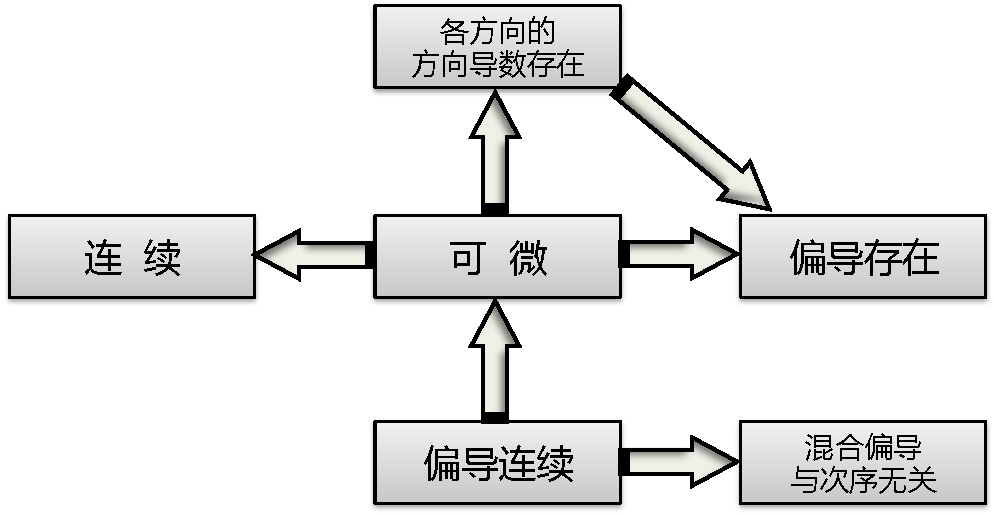
\includegraphics{./images/ch10/drela.pdf}} 
\end{center}

\begin{shaded}
{\bf 相关的反例}

1、连续但偏导不存在(连续但不可微)

$$f(x,y)=\sqrt{x^2+y^2}$$

2、偏导存在但不连续(偏导存在但不可微)

$$
f(x,y)=\left\{\begin{array}{ll}
0 & ,(x,y)=(0,0)\\
\df{xy}{x^2+y^2}& ,else
\end{array}\right.
$$

3、可微但偏导不连续

$$
f(x,y)=\left\{\begin{array}{ll}
0 & ,(x,y)=(0,0)\\
(x^2+y^2)\sin\df1{x^2+y^2}& ,else
\end{array}\right.
$$

4、偏导不连续且混合偏导数不相等

$$
f(x,y)=\left\{\begin{array}{ll}
0 & ,(x,y)=(0,0)\\
xy\df{x^2-y^2}{x^2+y^2}& ,else
\end{array}\right.
$$

5、连续、偏导存在且任意方向的方向导数(按同济教材的定义)均存在但不可微

$$
f(x,y)=\left\{\begin{array}{ll}
0 & ,(x,y)=(0,0)\\
\df{\sqrt{|xy|}}{x^2+y^2}\sin(x^2+y^2)& ,else
\end{array}\right.
$$

6、所有的方向导数(按KD教材的定义)存在而不可微

$$
f(x,y)=\left\{\begin{array}{ll}
0 & ,y=0\\
\df{x^2+y^2}{y}& ,else
\end{array}\right.
$$

7、方向导数(按同济教材的定义)满足$D_uf=f'_x\cos\theta+f'_y\sin\theta\;
(u=\rho\sin\theta)$但不可微,甚至不连续

$$
f(x,y)=\left\{\begin{array}{ll}
y=\rho\sin\theta & ,(x,y)\in D_1\\
1& ,(x,y)\in D_2\\
0& ,else
\end{array}\right.
$$
其中$D_1$为心形线$\rho=1-\cos\theta$及其内部,$D_2$表示其外部,且不在$x$轴上。

[提示]: $f'_x(0,0)=0,f'_y(0,0)=1,D_uf=\sin\theta$,在$D_2$
内总存在靠近$(0,0)$的某点,使得
$$|f(x,y)-f(0,0)-[f'_x(0,0)x+f'_y(0,0)y]|=1$$


\end{shaded}

\newpage

\section*{习题课}
\addcontentsline{toc}{section}{习题课}

\subsection*{多元函数的极限、连续、偏导数与全微分}

{\bf 辅导(下)-P12-例6-6:}讨论极限$\lim\limits_{(x,y)\to(0,0)}\df{xy^2}{x^2+y^4}$

$$\lim\limits_{x\to 0\atop{y=kx}}\df{xy^2}{x^2+y^4}=0$$

$$\lim\limits_{x\to 0\atop{y^2=x}}\df{xy^2}{x^2+y^4}=\df12$$

{\bf 辅导(下)-P12-例6-7:}证明极限$\lim\limits_{(x,y)\to(0,0)}(1+xy)
^{\frac1{x+y}}$不存在


$$\lim\limits_{x\to 0\atop{y=kx}}(1+xy)^{\frac1{x+y}}=1\quad (k\ne -1)$$

$$\lim\limits_{x\to 0\atop{y=x^2-x}}(1+xy)^{\frac1{x+y}}=e^{-1}$$

{\bf 辅导(下)-P12-例6-8:}证明极限$\lim\limits_{(x,y)\to(0,0)}
\df{x^3+xy^2}{x^2-xy+y^2}=0$

{\bf 例:}证明函数
  $$f(x,y)=\left\{\begin{array}{cc}
  	\df{x^2y}{x^2+y^2},& (x,y)\ne (0,0)\\
  	0,& else
  \end{array}\right.$$
  在原点可微,但偏导数不连续。

{\bf 辅导(下)-P16-例6-16:}证明:$z=\sqrt|xy|$在
原点连续,偏导数存在,但不可微。

{\bf 课后思考:}习题8.2:16-18

{\bf 辅导(下)-P17-例6-17:}正六棱台的上下底和高分别为$1,2,2$,问
那个值的测量误差对其侧面积的值影响最大?

$$S=6\times\df12(x+y)\times\df12\sqrt{4z^2+3(y-x)^2}$$

$$\d z|_{(1,2,2)}=S'_x(1,2,2)\Delta x+S'_y(1,2,2)\Delta y+
S'_z(1,2,2)\Delta z=\df3{\sqrt{19}}(5\Delta x+14\Delta y+12\Delta z)$$

\subsection*{复合函数求导}

{\bf 例:}
\begin{enumerate}[(1)]
  \setlength{\itemindent}{1cm}
  \item 设$z=u^2\ln v,u=\df xy,v=3x-2y$,求$\df {\p z}{\p x},\df{\p z}{\p
  y}$ 
  \item 设$z=\arctan(xy),y=e^x$,求$\df{\d z}{\d x}$ 
  \item 设$u=f\left(\df xy,\df yz\right)$,求$\df {\p u}{\p x},\df {\p u}{\p y}$
  和$\df {\p u}{\p z}$ 
  \item 设$f(x,2x)=x,f\,'_1(x,2x)=x^2$,求$f\,'_2(x,2x)$
\end{enumerate}

{\bf 例:}设$f(x,y)$一阶偏导连续,$f(1,1)=1,f\,'_x(1,1)=2$,
$f\,'_y(1,1)=3$,又$\varphi(x)=f(x,f(x,x))$,求
$$\left.\df{\d\varphi^3(x)}{\d x}\right|_{x=1}$$

{\bf 例:}设$z=xf\left(\df yx\right)+yg\left(x,\df xy\right)$,
其中$f,g$均二次可微,求$\df{\p^2 z}{\p x\p y}$

{\bf 例:}设$f(x,y)$一阶偏导数连续,且对任意实数$t$,有
$$f(tx,ty)=tf(x,y)$$
证明:曲面$z=f(x,y)$上任一点$M$处的切平面与向径平行。

\subsection*{隐函数求导}

{\bf 例:}设$z=z(x,y)$由方程$x^2+y^2+z^2=xf\left(\df yx\right)$确定,
且$f$可微,求$\df {\p z}{\p x},\df{\p z}{\p y}$

{\bf 例:}设$y=f(x,t)$,其中$t$是由$F(x,y,t)=0$所确定的隐函数,$f,F$具有
一阶连续偏导数,求$\df{\d y}{\d x}$

{\bf 例:}设$F(u,v)$具有一阶连续偏导数,且由$F\left(\df xz,\df yz\right)=0$
可确定函数$z=z(x,y)$,求$x\df{\p z}{\p x}+y\df{\p z}{\p y}$

{\bf 例:}设$u=u(x,y),x=r\cos\theta,y=r\sin\theta$,将方程
$$x\df{\p u}{\p y}-y\df{\p u}{\p x}=0$$
化为$u$关于$r,\theta$的偏导数的方程。

{\bf 例:}设$u=u(x,y,z)$具有连续偏导数,且
$$x=r\sin\theta\cos\varphi,y=r\sin\theta\sin\varphi,z=r\cos\theta$$
证明:若$x\df{\p u}{\p x}+y\df{\p u}{\p y}+z\df{\p u}{\p z}=0$,
则$u$与$r$无关。

{\bf 例:}设$f(x,y)$一阶偏导连续,$f(1,1)=1,f\,'_1(1,1)=a$,
$f\,'_2(1,1)=b$,又$\varphi(x)=f(x,f(x,f(x,x)))$,求
$\varphi(1)$与$\varphi'(1)$。

{\bf 例:}设由$\ln(xz)+\arctan(yz)=0$可确定隐函数$z=z(x,y)$,求$z'_x$。

{\bf 辅导(下)-P21-例6-26:}设$u=u(x)$由
$$u=f(x,y),\;g(x,y,z)=0,\;h(x,z)=0$$
确定,$f,g,h$一阶偏导连续,$h'_z\ne0,g'_y\ne0$,求$\df{\p u}{\p x}$

$$u'_x=f'_x-\df{f'_yg'_x}{g'_y}+\df{f'_yg'_zh'_x}{g'_yh'_z}$$

\subsection*{方向导数}

{\bf 例:}求函数$z=x^2-xy+y^2$在点$(1,1)$处沿与$x$轴正向成
$\alpha$角的方向$\bm{l}$的方向导数。在怎样的方向上
此导数取最大、最小及$0$值?

{\bf 例:}设$u=u(x,y,z)$,证明:$u$为$x,y,z$的线性函数,当且仅当
$\bigtriangledown u$为常矢量。

{\bf 例:}试证曲面$\sqrt{x}+\sqrt y+\sqrt z=\sqrt a\,(a>0)$
在任一点处的切平面在三个坐标轴上的截距之和为常数。

{\bf 例:}已知曲面方程$z=xe^{y/x}$,证明:曲面上任一点$M$处的法线与其
向径垂直。

\subsection*{Taylor公式}

{\bf 例:}试证明:当$x,y$很小时,有如下近似公式:
$$(1+x)^m(1+y)^n\approx 1+mx+ny$$

{\bf 例:}试证明:当$x,y$很小时,有如下近似公式:
\begin{enumerate}[(1)]
  \setlength{\itemindent}{1cm}
  \item $\ln(1+x)\ln(1+y)\approx xy$
  \item $\arctan\df{x+y}{1+xy}\approx x+y$
\end{enumerate}

\subsection*{极值与条件极值}

{\bf 辅导(下)-P28-例6-39:}求以$(0,0),(0,1),(1,0)$为顶点的三角形区域内
到该三点距离平方和最大的点。

{\bf 例:}证明函数$f(x,y)=2x^2-3xy^2+y^4$不存在极值。

{\bf 例:}当$x,y,z$均大于零时,求函数$u=\ln x+2\ln y+3\ln z$
在球面$x^2+y^2+z^2=6R^2$上的最大值,并证明对任意正数
$a,b,c$,成立不等式
$$ab^2c^3\leq 108\left(\df{a+b+c}{6}\right)^6$$

[解]:由Lagrange乘子法,记
$$L=xy^2z^3+\lambda(x^2+y^2+z^2-6R^2),$$
令$\bigtriangledown L=0$,可解得$x=R,y=\sqrt2 R,z=\sqrt3 R$,从而有:
$$xy^2z^3\leq 6\sqrt 3R^6=6\sqrt 3\left(\df{x^2+y^2+z^2}{6}\right)^3.$$
也即
$$x^2y^4z^6\leq 108\left(\df{x^2+y^2+z^2}{6}\right)^6.$$
记$a=x^2,b=y^2,c=z^2$,即证。

[提示]:使用Lagrange乘子法求解该题有不小的计算量,事实上,也可以直接使用平均值不等式
的方法来求解。

注意到$a,b,c>0$时
$$\df{a+b+c}6=\df16\left(a+\df b2+\df b2+\df c3+\df c3+\df c3\right)
\geq \sqrt[6]{\df{ab^2c^3}{108}},$$
稍加整理即为第二问的不等式(当且仅当$a=\df b2=\df c3$时,等号成立)。

记$a=x^2,b=y^2,c=z^2$,则由上式,当$x^2+y^2+z^2=6R^2$时,有
$$x^2y^4z^6\leq108\left(\df{x^2+y^2+z^2}{6}\right)^6
=108\left(R^2\right)^6$$
进而\ps{\b 求解极值和条件极值问题,不应拘泥于Lagrange乘子法的“套路”,合理地
使用已经熟悉的不等式,常常能够使计算大为简化}
$$xy^2z^3\leq6\sqrt3R^6.$$
并且,我们容易知道当且仅当$x^2=\df{y^2}2=\df{z^2}3$时,取到以上的最大值。

{\bf 例:}在半径为$R$的圆的内接三角形中,求面积最大者。

[提示]:圆的内接三角形的面积由圆的半径$r$和各边对应的圆心角$\alpha,\beta,\gamma$
确定,具体地
$$S=\df{r^2}2(\sin\alpha+\sin\beta+\sin\gamma),\quad
(\alpha+\beta+\gamma=2\pi)$$
如果不使用Lagrange乘子法,利用变量替换$\gamma=2\pi-\alpha-\beta$,则
\begin{align*}
	\sin\alpha+\sin\beta+\sin\gamma
	&=2\sin\df{\alpha+\beta}2\cos\df{\alpha-\beta}2-\sin(\alpha+\beta)\\
	&=2\sin\df{\alpha+\beta}2\cos\df{\alpha-\beta}2-2\sin\df{\alpha+\beta}2
	\cos\df{\alpha+\beta}2\\
	&=2\sin\df{\alpha+\beta}2\left(\cos\df{\alpha-\beta}2
	-\cos\df{\alpha+\beta}2\right)\\
	&=4\sin\df{\alpha+\beta}2\sin\df{\alpha}2\sin\df{\beta}2
	\quad(0\leq\alpha+\beta\leq2\pi)
\end{align*}
这样问题就转换成了求解二元函数$\sin\df{\alpha+\beta}2\sin\df{\alpha}2\sin\df{\beta}2$
在闭区域$0\leq\alpha+\beta\leq2\pi$上的极值问题,接下来还会有相当大的计算量。

如果使用Lagrange乘子法,则可设\ps{\b 这个例子说明,使用Lagrange乘子法,并不一定总是
计算量很大,所以我们应该尽可能考虑综合使用各种可行的方法}
$$L=\sin\alpha+\sin\beta+\sin\gamma+\lambda(\alpha+\beta+\gamma-2\pi),$$
于是$\bigtriangledown L=0$也即
$$
	\left\{\begin{array}{l}
		\cos\alpha+\lambda=0\\
		\cos\beta+\lambda=0\\
		\cos\gamma+\lambda=0\\
		\alpha+\beta+\gamma-2\pi=0
	\end{array}\right.
$$
观察方程组的特点,容易发现$\alpha=\beta=\gamma$时取极值,计算量较前面的方法大为减少。

{\bf 例:}现有资金$36$元,要建造一个无盖的长方体容器,已知底面造价为$3$元每平方米,
侧面造价为$1$元每平方米,求可造出的长方体的最大容积。
		
{\bf 例:}证明函数$f(x,y)=e^{\cos x}-y^2$在全平面上有无穷多个
极大值,但无极小值。

[提示]:如图\ps{对可微的一元函数而言,两个极大值点之间必有至少一个极小值点,对多元函数则不然!}
\begin{center}
	\resizebox{!}{5cm}{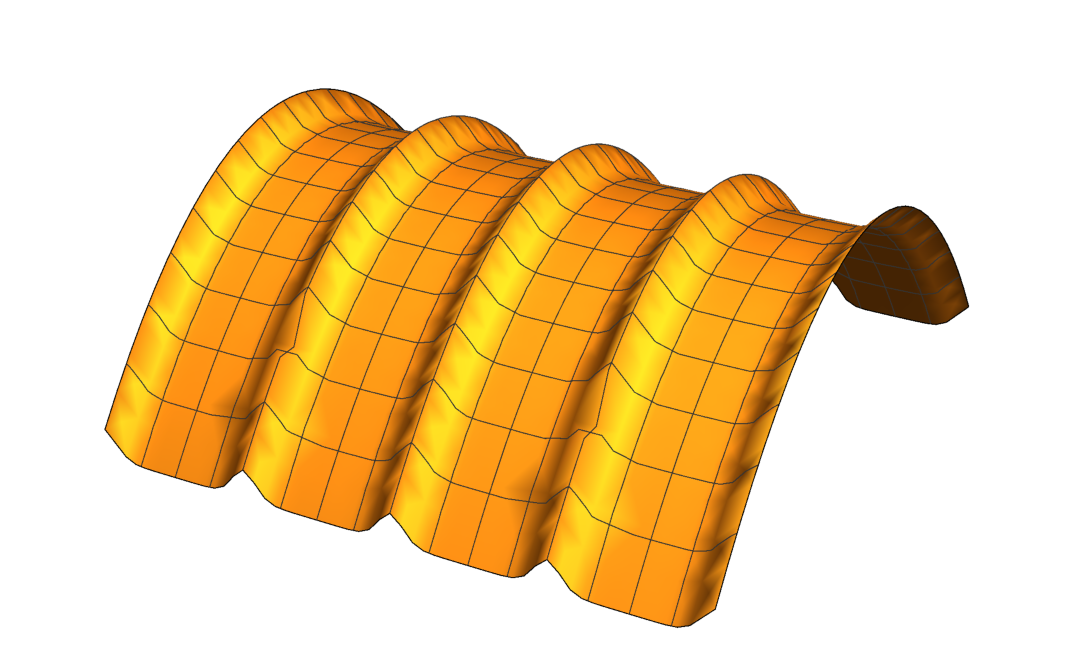
\includegraphics{./images/ch10/iUnD.pdf}}
\end{center}

{\bf 例:}设$F(x,y,z)$在条件$\varphi(x,y,z)=0$和$\psi(x,y,z)=0$
之下在点$P_0(x_0,y_0,z_0)$处取得极值$m$,证明:曲面
$F(x,y,z)=m,\varphi(x,y,z)=0$和$\psi(x,y,z)=0$
在$P_0$的法线共面,其中函数$F,\varphi,\psi$均有连续且不同时
为零的一阶偏导数。

{\bf 例:}求函数$z=x^2-xy+y^2$在区域$D:|x|+|y|\leq 1$
上的最大和最小值。

[提示]:令$x+y=X,x-y=Y$,则\ps{任意形如$ax^2+bxy+cy^2$的函数都可以通过
该线性变换化为形如$AX^2+BY^2$的形式!}
$$z=x^2-xy+y^2=\df14X^2+\df34Y^2,$$
$$D:|x|+|y|\leq 1\quad\Leftrightarrow\quad |X|\leq1,|Y|\leq1$$
易知$|X|=|Y|=1$时,$z$取最大值$1$,$|X|=|Y|=0$时,$z$取最大值$0$.

如果使用普通的方法,计算量会大很多。

\subsection*{课堂思考}

{\bf 例:}设$F(x,y)=\dint_0^{xy}\df{\sin t}{1+t^2}\d t$,则
$\left.\df{\p^2F}{\p x^2}\right|_{x=0 \atop y=2}=$
\underline{\quad\quad\quad}

{\bf 例:}设$z=f(xy,yg(x))$,其中$f$二阶偏导数连续,$g(x)$可导且
有极值$g(1)=1$,求$\left.\df{\p^2z}{\p x\p y}\right|_{x=1\atop y=1}$

\section*{习题参考解答}
\addcontentsline{toc}{section}{习题参考解答}

\begin{center}
	\bf 9.1 多元函数的极限与连续
\end{center}

1.讨论以下二重极限的存在性
\begin{enumerate}[(1)]
  	\setlength{\itemindent}{1cm}
    \item $\lim\limits_{(x,y)\to(0,0)}\df{x+y}{\sqrt{x^2+y^2}}$
%     \item $\lim\limits_{(x,y)\to(0,0)}\df{y^2+\sin x}{y^2+x}$
    \item $\lim\limits_{(x,y)\to(0,0)}\df{xy}{|x|+|y|}$
  \end{enumerate}

[解]:(1)令$x=\rho\cos\theta,y=\rho\sin\theta$,则
$$\lim\limits_{(x,y)\to(0,0)}\df{x+y}{\sqrt{x^2+y^2}}
=\lim\limits_{\rho\to 0}(\cos\theta+\sin\theta)=\cos\theta+\sin\theta,$$
注意到右端结果与$\theta$相关,故该二重极限不存在。

(2)令$x=\rho\cos\theta,y=\rho\sin\theta$,则
$$\lim\limits_{(x,y)\to(0,0)}\df{xy}{|x|+|y|}
=\lim\limits_{\rho\to0}\df{\rho\cos\theta\sin\theta}{|\cos\theta|+|\sin\theta|},$$
注意到$|\cos\theta|+|\sin\theta|\geq\sqrt2$,故对任意$\e>0$,令
$\delta=\sqrt2\e$,则对任意$0<|\rho|<\delta$,总有
$$\left|\df{\rho\cos\theta\sin\theta}{|\cos\theta|+|\sin\theta|}\right|
\leq\df{\rho}{\sqrt2}<\e,$$
由此可知,该二重极限存在。\fin

2.计算以下二重极限
\begin{enumerate}[(1)]
    \setlength{\itemindent}{1cm}
    \item $\lim\limits_{(x,y)\to(0,1)}\df{\ln(1+xy)}{y\sin x}$
    \item $\lim\limits_{(x,y)\to(0,0)}\df{1-\cos(xy)}{(x^2+y^2)e^{x^2}}$
    \item $\lim\limits_{(x,y)\to(0,0)}\df{e^{xy}-1}{\sqrt{2-e^{xy}}-1}$
  \end{enumerate}

[解]:提示:以下计算过程中使用了等价无穷小代换

(1)
$\lim\limits_{(x,y)\to(0,1)}\df{\ln(1+xy)}{y\sin x}
=\lim\limits_{(x,y)\to(0,1)}\df{xy}{yx}=1.$

(2)
$\lim\limits_{(x,y)\to(0,0)}\df{1-\cos(xy)}{(x^2+y^2)e^{x^2}}
=\lim\limits_{(x,y)\to(0,0)}\df{\frac12x^2y^2}{(x^2+y^2)}
=\df12\lim\limits_{x\to 0}\lim\limits_{y\to0}\df{x^2y^2}{x^2+y^2}=0.$

(3)
$\lim\limits_{(x,y)\to(0,0)}\df{e^{xy}-1}{\sqrt{2-e^{xy}}-1}
=\lim\limits_{(x,y)\to(0,0)}\df{xy}{\frac12(1-e^{xy})}
=-2\lim\limits_{(x,y)\to(0,0)}\df{xy}{xy}=-2.$
\fin

\bs

\begin{center}
	\bf 9.2 偏导数与全微分
\end{center}

1.证明:函数$f(x,y)=\left\{\begin{array}{ll}
  	(x^2+y^2)\sin\df1{x^2+y^2}, & (x,y)\ne(0,0)\\
  	0, & (x,y)=(0,0)
  \end{array}\right.$
  的偏导函数在原点处不连续,但$f(x,y)$在原点处可微。

[解]:由偏导数的定义,
$$f'_x(0,0)=\lim\limits_{\Delta x\to 0}
\df{(\Delta x)^2\sin\frac1{(\Delta x)^2}}{\Delta x}=0,$$
同理可得$f'_x(0,0)=0$。

又当$(x,y)\ne(0,0)$时,由偏导数的求导法则,可得
$$f'_x(x,y)=2x\sin\df1{x^2+y^2}-\df{2x}{x^2+y^2}\cos\df1{x^2+y^2},$$
$$f'_y(x,y)=2y\sin\df1{x^2+y^2}-\df{2y}{x^2+y^2}\cos\df1{x^2+y^2},$$
注意到累次极限
$$\lim\limits_{x\to 0}\lim\limits_{y\to 0}
f'_x(x,y)
=\lim\limits_{x\to 0}
\left[2x\sin\df1{x^2}-\df{2}{x}\cos\df1{x^2}\right]
=-\lim\limits_{x\to 0}
\df{2}{x}\cos\df1{x^2}$$
不存在,故二重极限$\lim\limits_{(x,y)\to(0,0)}f'_x(x,y)$
不存在,从而可知偏导函数$f'_x(x,y)$在原点处不连续。

同理可证$f'_y(x,y)$在原点处不连续。

进一步,注意到极限
\begin{align*}
	&\lim\limits_{(x,y)\to(0,0)}\df{f(\Delta x,\Delta y)-f'_x(0,0)\Delta x
	-f'_y(0,0)\Delta y}{\sqrt{(\Delta x)^2+(\Delta y)^2}}\\
	&=\lim\limits_{(x,y)\to(0,0)}\sqrt{(\Delta x)^2+(\Delta y)^2}
	\sin\df1{(\Delta x)^2+(\Delta y)^2}=0,
\end{align*}
故
$$f(\Delta x,\Delta y)-f'_x(0,0)\Delta x-f'_y(0,0)\Delta y
=\circ(\sqrt{(\Delta x)^2+(\Delta y)^2}),$$
也即$f(x,y)$在原点处可微。\fin

\bs

% 2.求$z=e^x\sin(x+y)$的所有二阶偏导数。
% 
% [解]:
% \begin{align*}
% 	z'_x&=e^x[\sin(x+y)+\cos(x+y)],\\
% 	z'_y&=e^x\cos(x+y),\\
% 	z''_{xx}&=2e^x\cos(x+y),\\
% 	z''_{yy}&=-e^x\sin(x+y),\\
% 	z''_{xy}&=z''_{yx}=e^x[\cos(x+y)-\sin(x+y)].
% \end{align*}
% \fin

2.求$z=\arctan\df{x+y}{1-xy}$的所有二阶偏导数。

[解]:注意到
$$\arctan\df{x+y}{1-xy}=\arctan x+\arctan y,$$
故
\begin{align*}
	z'_x&=\df1{1+x^2},\\
	z'_y&=\df1{1+y^2},\\
	z''_{xx}&=-\df{2x}{(1+x^2)^2},\\
	z''_{yy}&=-\df{2y}{(1+y^2)^2},\\
	z''_{xy}&=z''_{yx}=0.
\end{align*}
\fin

\bs

3.已知$\df{\p z}{\p y}=\df{x^2+y^2}y$,$z(x,1)=e^x$,
求$z(x,y)\;(y\ne0)$。

[解]:由$\df{\p z}{\p y}=\df{x^2+y^2}y=\df{x^2}y+y$,可知
$$z(x,y)=x^2\ln|y|+\df12y^2+u(x),$$
其中$u(x)$是某个关于$x$的一元函数。又$z(x,1)=e^x$,也即
$$e^x=\df12+u(x)\quad
\Rightarrow\quad u(x)=e^x-\df12,$$
故
$$z(x,y)=x^2\ln|y|+\df12(y^2-1)+e^x.$$
\fin

\bs

4.设$z=\dint_x^{xy}e^{(t-x)^2}\d t$,求$\df{\p z}{\p x}$和$\df{\p z}{\p y}$。

[解]:令$u=t-x$,则
$$z=\dint_0^{x(y-1)}e^{u^2}\d u.$$
进而
$$
	z'_x=(y-1)e^{x^2(y-1)^2},\quad z'_y=xe^{x^2(y-1)^2}.
$$
\fin

\bs

5.求函数$z=xy^2$在$(1,2)$附近且$(\Delta x,\Delta y)=(0.1,-0.5)$时
对应的函数值的改变量(全增量)与全微分。

[解]:全增量
$$\Delta z=z(1.1,1.5)-z(1,2)=-1.525,$$
注意到$z'_x(1,2)=z'_y(1,2)=4$,故全微分
$$\d z=z'_x(1,2)\Delta x+z'_y(1,2)\Delta y
=4\cdot 0.1+4\cdot(-0.5)=-1.6.$$
\fin

\bs

6.利用微分计算$\sqrt{1.02+(1.97)^3}$的近似值。

[解]:考虑函数$z=\sqrt{x+y^3}$,则
$$z(1,2)=3,\quad z'_x(1,2)=\df16,\quad z'_y(1,2)=2.$$
进而可知
$$\sqrt{1.02+(1.97)^3}
\approx z(1,2)+z'_x(1,2)\cdot0.02+z'_y(1,2)\cdot(-0.03)
\approx 2.943.$$
\fin

\bs

\begin{center}
	\bf 9.3 多元复合函数与隐函数的偏导数
\end{center}

1.设$u=f\left(\df xy,\df yz\right)$,求$\df {\p u}{\p x},\df {\p u}{\p y}$
和$\df {\p u}{\p z}$。

[解]:
\begin{align*}
	u'_x&=f'_1\left(\df xy,\df yz\right)\df1y,\\
	u'_y&=-f'_1\left(\df xy,\df yz\right)\df x{y^2}
	+f'_2\left(\df xy,\df yz\right)\df1z,\\
	u'_x&=-f'_2\left(\df xy,\df yz\right)\df{y}{z^2}.
\end{align*}
\fin

\bs

2.设$f(x,y)$一阶偏导连续,$f(1,1)=1,f\,'_x(1,1)=2$,
$f\,'_y(1,1)=3$,又$\varphi(x)=f(x,f(x,x))$,求
$\left.\df{\d\varphi^3(x)}{\d x}\right|_{x=1}$。

[解]:
$$\varphi'(1)=f'_x(1,f(1,1))+f'_y(1,f(1,1))[f'_x(1,1)+f'_y(1,1)]
=17,$$
进而
\begin{align*}
	\left.\df{\d\varphi^3(x)}{\d x}\right|_{x=1}
	&=\left.3\varphi^2(x)\varphi'(x)\right|_{x=1}=51.
\end{align*}
\fin

\bs

3.设$z=xf\left(\df yx\right)+yg\left(x,\df xy\right)$,
其中$f,g$均二次可微,求$\df{\p^2 z}{\p x\p y}$。

[解]:
\begin{align*}
	z'_x&=f\left(\df yx\right)-f'\left(\df yx\right)\df{y}{x^2}
	+y\left[g'_1\left(x,\df xy\right)+g'_2\left(x,\df xy\right)\df1y\right],\\
	z''_{xy}&=f'\left(\df yx\right)\df1x
	-f''\left(\df yx\right)\df{y}{x^3}-f'\left(\df yx\right)\df1{x^2}
	+g'_1\left(x,\df xy\right)+g'_2\left(x,\df xy\right)\df1y\\
	&\quad
	y\left[-g''_{12}\left(x,\df xy\right)\df{x}{y^2}-g''_{22}\left(x,\df
	xy\right)\df{x}{y^3}-g'_2\left(x,\df xy\right)\df1{y^2}\right].
\end{align*}
\fin

\bs

4.设$f(x,y)$一阶偏导数连续,且对任意实数$t$,有
$$f(tx,ty)=tf(x,y),$$
证明:曲面$z=f(x,y)$上任一点$M$处的切平面与向径平行。

[解]:已知等式两边关于$t$求导,可得
$$f'_1(tx,ty)x+f'_2(tx,ty)y=f(x,y),$$
令$t=1$,整理后可得
$$(f'_x(x,y),f'_y(x,y),-1)\cdot(x,y,f(x,y))=0,$$
注意到$(f'_x(x,y),f'_y(x,y),-1)$为曲面上一点$(x,y,f(x,y))$处的法向量,从而
可知曲面在该点处的切平面必与其该点的相近平行。\fin

5.设$F(u,v)$具有一阶连续偏导数,且由$F\left(\df xz,\df yz\right)=0$
可确定函数$z=z(x,y)$,求$x\df{\p z}{\p x}+y\df{\p z}{\p y}$。

[解]:对$F\left(\df xz,\df yz\right)=0$两边求微分,可得
$$F'_1\left(\df xz,\df yz\right)\left(\df1z\d x-\df x{z^2}\d z\right)
+F'_2\left(\df xz,\df yz\right)\left(\df1z\d y
-\df{y}{z^2}\d z\right)=0,$$
由此可得
$$
z'_x=\df{zF'_1}{xF'_1+yF'_2},\quad
z'_y=\df{zF'_2}{xF'_1+yF'_2},
$$
进而可得
$$x\df{\p z}{\p x}+y\df{\p z}{\p y}=z.$$
\fin

\bs

6.设$y=f(x,t)$,其中$t$是由$F(x,y,t)=0$所确定的隐函数,$f,F$具有
一阶连续偏导数,求$\df{\d y}{\d x}$。

[解]:在$y=f(x,t)$和$F(x,y,t)=0$两边同时求微分,可得
$$
	\left\{\begin{array}{l}
		\d y=f'_1\d x+f'_2\d t,\\
		F'_1\d x+F'_2\d y+F'_3\d t=0.
	\end{array}\right.
$$
消去$\d t$,整理后可得
$$\df{\d y}{\d x}=\df{f'_2F'_1+f'_1F'_3}{F'_3-f'_2F'_2}.$$
\fin

7.设$u=u(x,y),x=r\cos\theta,y=r\sin\theta$,将方程
$$x\df{\p u}{\p y}-y\df{\p u}{\p x}=0$$
化为$u$关于$r,\theta$的偏导数的方程。

[解]:由已知$r=\sqrt{x^2+y^2},\theta=\arctan\df yx$,从而
$$
	r'_x=\df xr,\quad r'_y= \df yr,\quad
	\theta'_x=-\df y{r^2},\quad \theta'_y=\df x{r^2}. 
$$
从而
\begin{align*}
	u'_x&=u'_rr'_x+u'_{\theta}\theta'_x=\df{u'_rxr-u'_{\theta}y}{r^2},\\
	u'_y&=u'_rr'_y+u'_{\theta}\theta'_y=\df{u'_ryr+u'_{\theta}x}{r^2}.
\end{align*}
于是
$$x\df{\p u}{\p y}-y\df{\p u}{\p x}=u'_{\theta},$$
进而可知原方程可化为$u'_{\theta}=0$。\fin

\bs

\begin{center}
	\bf 方向导数、梯度、Hessian矩阵与多元Taylor公式
\end{center}

1.求曲面$z=x^2+y^2$上的点$(1,1,2)$处沿椭圆$\df{x^2}{8}+\df{y^2}{2}=1$
在$(2,1)$的外法向的方向导数。

[解]:由梯度的几何意义,椭圆$\df{x^2}{8}+\df{y^2}{2}=1$在$(2,1)$的外法向为
$\bm{u}=\left(\df12,1\right)$。从而所求方向导数
$$D_uz(1,1,2)=\bm{e}_u\cdot\bigtriangledown z(1,1)
=\left(\df1{\sqrt5},\df2{\sqrt5}\right)\cdot (2,2)=\df6{\sqrt5}.$$
\fin

\bs

2.试证曲面$\sqrt{x}+\sqrt y+\sqrt z=\sqrt a\,(a>0)$
在任一点处的切平面在三个坐标轴上的截距之和为常数。

[证]:任取曲面上一点$(x_0,y_0,z_0)$,则曲面该点处的法向量为
$$\bm{n}=\left(\df1{\sqrt{x_0}},\df1{\sqrt{y_0}},
\df1{\sqrt{z_0}}\right),$$
从而切平面为
$$\df1{\sqrt{x_0}}(x-x_0)+\df1{\sqrt{y_0}}(y-y_0)
+\df1{\sqrt{z_0}}(z-z_0)=0,$$
其在三个坐标轴上的截距分别为$a\sqrt{x_0},a\sqrt{y_0},a\sqrt{z_0}$,
由此易知结论成立。\fin

\bs

3.已知曲面方程$z=xe^{y/x}$,证明:曲面上任一点$M$处的法线与其
向径垂直。

[证]:曲面上任一点$(x,y,z)$处的法向量为
$$\bm{n}=\left(e^{y/x}(1-\frac yx,e^{y/x},-1\right),$$
向径为$\bm{r}=(x,y,z)$,容易验证$\bm{n}\cdot\bm{r}=0$。\fin

\bs

4.求函数$xe^{x+y}$在原点处带Peano余项的二阶Taylor公式。

[解]:
$$xe^{x+y}=x+x^2+xy+\circ(x^2+y^2).$$
\fin

\bs

\begin{center}
	\bf 9.5 多元函数的极值与条件极值
\end{center}

1.求内接于椭球面$\df{x^2}{a^2}+\df{y^2}{b^2}+\df{z^2}{c^2}=1$
的长方体的最大体积。

[解]:设$(x,y,z)$为第一卦限内的椭球面上任一点,则以之为顶点的长方体体积为
$V=8xyz$。由平均值不等式,
$$\sqrt[3]{\df{x^2y^2z^2}{a^2b^2c^2}}
\leq\df13\left(\df{x^2}{a^2}+\df{y^2}{b^2}+\df{z^2}{c^2}\right)=\df13,$$
且当$\df{x^2}{a^2}=\df{y^2}{b^2}=\df{z^2}{c^2}$时取等号,从而可知
$$V\leq\df{(abc)^{\frac32}}{3\sqrt3},$$
也即椭球的最大内接长方体体积为$\df{(abc)^{\frac32}}{3\sqrt3}$,此时
$x=\df{a}{\sqrt3},y=\df{b}{\sqrt3},z=\df{c}{\sqrt3}$。\fin

\bs

2.某公司的产品广告有电台和报纸两种发布途径,经研究发现,产品销售收入$U$(万元)与
  投入的电台广告费用$T$(万元)和投入的报纸广告费用$P$(万元)满足如下关系
  $$U=15+14T+32P-8TP-2T^2-10P^2.$$
  \begin{enumerate}[(1)]
    \item 在广告预算不封顶的情况下,求公司的最优广告策略;
    \item 若广告总预算上限为$1.5$万元,求公司的最优广告策略。
  \end{enumerate}

[解]:(1)由已知可得
$$\bigtriangledown U=(14-8P-4T,32-8T-20P),$$
令$\bigtriangledown U=0$,可解得$P=1,T=1.5$。又
$$\bigtriangledown^2U=\left[\begin{array}{cc}
	-4 & -8 \\ -8 & -20
\end{array}\right]$$
是负定的,故可知此时公司的最优广告策略为电视广告投入$1$万元,
报纸广告投入$1.5$万元。

(2)注意到驻点$(1,1.5)$不超出了预算上限,故此时只需考虑取值区域
$$0\leq T\leq T+P\leq 1.5$$
边界上的极值问题。

当$T=0,0\leq P\leq 1.5$时,$U=15+32P-10P^2$,
易得其最大值为$40.5$,对应地$P=1.5$;

当$P=0,0\leq T\leq 1.5$时,$U=15+14T-2T^2$,易得其最大值为
$31.5$,对应地$T=1.5$;

当$0\leq T\leq T+P=1.5$时,$U=4(10.125-T^2)$,易得其最大值为
$40.5$,此时$T=0,P=1.5$。

综上可知,在广告预算上限为$1.5$万元时,最佳的广告投入策略是
全部投入报纸广告。\fin

\bs

3.已知$\lim\limits_{(x,y)\to(0,0)}\df{f(x,y)-4xy}{x^2+y^2}=1$,
判断$(0,0)$是否为$f(x,y)$的极值点,若是,是极大值还是极小值?

[解]:由已知可得
$$f(x,y)=4xy+x^2+y^2+\circ(x^2+y^2),$$
进而可知
$$\bigtriangledown f(0,0)=(0,0),\quad
\bigtriangledown^2f(0,0)=\left[\begin{array}{cc}
	1 & 2 \\ 2 & 1
\end{array}\right],$$
由此易知原点为$f(x,y)$的鞍点。\fin

\begin{ext}
	{\bf 课后作业}
	\begin{enumerate}
	  \item 求内接于椭球面$\df{x^2}{a^2}+\df{y^2}{b^2}+\df{z^2}{c^2}=1$
	  的长方体的最大体积。
	  \item 某公司的产品广告有电台和报纸两种发布途径,经研究发现,产品销售收入$U$(万元)与
	  投入的电台广告费用$T$(万元)和投入的报纸广告费用$P$(万元)满足如下关系
	  $$U=15+14T+32P-8TP-2T^2-10X^2.$$
	  \begin{enumerate}[(1)]
	    \item 在广告预算不封顶的情况下,求公司的最优广告策略;
	    \item 若广告总预算上限为$1.5$万元,求公司的最优广告策略。
	  \end{enumerate}
	  \item 已知$\lim\limits_{(x,y)\to(0,0)}\df{f(x,y)-4xy}{x^2+y^2}=1$,
	  判断$(0,0)$是否为$f(x,y)$的极值点,若是,是极大值还是极小值?
	\end{enumerate}
\end{ext}